%definira klasu dokumenta 
\documentclass[12pt]{report} 

%prostor izmedu naredbi \documentclass i \begin{document} se zove uvod. U njemu se nalaze naredbe koje se odnose na cijeli dokument

%osnovni LaTex ne može riješiti sve probleme, pa se koriste različiti paketi koji olakšavaju izradu željenog dokumenta
\usepackage[croatian]{babel} 
\usepackage{amssymb}
\usepackage{amsmath}
\usepackage{txfonts}
\usepackage{mathdots}
\usepackage{titlesec}
\usepackage{array}
\usepackage{lastpage}
\usepackage{etoolbox}
\usepackage{tabularray}
\usepackage{color, colortbl}
\usepackage{adjustbox}
\usepackage{geometry}
\usepackage[classicReIm]{kpfonts}
\usepackage{hyperref}
\usepackage{fancyhdr}

\usepackage{float}
\usepackage{setspace}
\restylefloat{table}


\patchcmd{\chapter}{\thispagestyle{plain}}{\thispagestyle{fancy}}{}{} %redefiniranje stila stranice u paketu fancyhdr

%oblik naslova poglavlja
\titleformat{\chapter}{\normalfont\huge\bfseries}{\thechapter.}{20pt}{\Huge}
\titlespacing{\chapter}{0pt}{0pt}{40pt}


\linespread{1.3} %razmak između redaka

\geometry{a4paper, left=1in, top=1in,}  %oblik stranice

\hypersetup{ colorlinks, citecolor=black, filecolor=black, linkcolor=black,	urlcolor=black }   %izgled poveznice


%prored smanjen između redaka u nabrajanjima i popisima
\newenvironment{packed_enum}{
	\begin{enumerate}
		\setlength{\itemsep}{0pt}
		\setlength{\parskip}{0pt}
		\setlength{\parsep}{0pt}
	}{\end{enumerate}}

\newenvironment{packed_item}{
	\begin{itemize}
		\setlength{\itemsep}{0pt}
		\setlength{\parskip}{0pt}
		\setlength{\parsep}{0pt}
	}{\end{itemize}}


%boja za privatni i udaljeni kljuc u tablicama
\definecolor{LightBlue}{rgb}{0.9,0.9,1}
\definecolor{LightGreen}{rgb}{0.9,1,0.9}

%Promjena teksta za dugačke tablice
\DefTblrTemplate{contfoot-text}{normal}{Nastavljeno na idućoj stranici}
\SetTblrTemplate{contfoot-text}{normal}
\DefTblrTemplate{conthead-text}{normal}{(Nastavljeno)}
\SetTblrTemplate{conthead-text}{normal}
\DefTblrTemplate{middlehead,lasthead}{normal}{Nastavljeno od prethodne stranice}
\SetTblrTemplate{middlehead,lasthead}{normal}

%podesavanje zaglavlja i podnožja

\pagestyle{fancy}
\lhead{Programsko inženjerstvo}
\rhead{Ozdravi} %naziv projektnog zadatka?
\lfoot{Welebyte}
\cfoot{stranica \thepage/\pageref{LastPage}}
\rfoot{\today}
\renewcommand{\headrulewidth}{0.2pt}
\renewcommand{\footrulewidth}{0.2pt}


\begin{document} 
	\begin{titlepage}
		\begin{center}
			\vspace*{\stretch{1.0}} %u kombinaciji s ostalim \vspace naredbama definira razmak između redaka teksta
			\LARGE Programsko inženjerstvo\\
			\large Ak. god. 2023./2024.\\
			
			\vspace*{\stretch{3.0}}
			
			\huge $$Ozdravi$$\\
			\Large Dokumentacija, Rev. \textit{$1.2$}\\
			
			\vspace*{\stretch{12.0}}
			\normalsize
			Grupa: \textit{Welebyte}\\
			Voditelj: \textit{Dorian Matić}\\
			
			
			\vspace*{\stretch{1.0}}
			%Datum predaje: \textit{$<$17$>$. $<$studenoga$>$. $<$2023$>$.}\\
			Datum predaje: \textit{17. studenoga 2023.}\\
	
			\vspace*{\stretch{4.0}}
			
			Nastavnik: \textit{Ivana Lulić}\\
		
		\end{center}

	
	\end{titlepage}

	\tableofcontents

	\chapter{Dnevnik promjena dokumentacije}
		
		\textbf{\textit{Kontinuirano osvježavanje}}\\
				
		
		\begin{longtblr}[
				label=none
			]{
				width = \textwidth, 
				colspec={|X[2]|X[13]|X[3]|X[4]|}, %sirina celije []
				rowhead = 1
			}
			\hline
			\textbf{Rev.}	& \textbf{Opis promjene/dodatka} & \textbf{Autori} & \textbf{Datum}\\[3pt] \hline
			0.1 & Napravljen predložak.	& L. Crvelin & 24.10.2023. 		\\[3pt] \hline 
            0.2	& Napisan opis projektnog zadatka. & L. Crvelin & 27.10.2023. 	\\[3pt] \hline
            0.3.1	& Napisani funkcionalni zahtjevi. & L. Crvelin & 27.10.2023. 	\\[3pt] \hline
            0.3.2	& Izmijenjeni funkcionalni zahtjevi. & L. Crvelin & 31.10.2023. 	\\[3pt] \hline
            0.4.1	& Dodani opisi obrazaca uporabe. & L. Crvelin & 2.11.2023. 	\\[3pt] \hline 
			0.4.2   & Dovršeni opisi obrazaca uporabe. & * & dd.mm.2023. \\ [3pt] \hline 
			0.2	& Dopisane upute za povijest dokumentacije.\newline Dodane reference. & * & dd.mm.2023. 	\\[3pt] \hline 
			0.5 & Dodan \textit{Use Case} dijagram i jedan sekvencijski dijagram, funkcionalni i nefunkcionalni zahtjevi i dodatak A & * & dd.mm.2023. \\[3pt] \hline 
			0.6 & Arhitektura i dizajn sustava, algoritmi i strukture podataka & * & dd.mm.2023. \\[3pt] \hline 
			0.8 & Povijest rada i trenutni status implementacije,\newline Zaključci i plan daljnjeg rada & * & dd.mm.2023. \\[3pt] \hline 
			0.9 & Opisi obrazaca uporabe & * & dd.mm.2023. \\[3pt] \hline 
			0.10 & Preveden uvod & * & dd.mm.2023. \\[3pt] \hline 
			0.11 & Sekvencijski dijagrami & * & dd.mm.2023. \\[3pt] \hline 
			0.12.1 & Započeo dijagrame razreda & * & dd.mm.2023. \\[3pt] \hline 
			0.12.2 & Nastavak dijagrama razreda & * & dd.mm.2023. \\[3pt] \hline 
			\textbf{1.0} & Verzija samo s bitnim dijelovima za 1. ciklus & * & dd.mm.2023. \\[3pt] \hline 
			1.1 & Uređivanje teksta -- funkcionalni i nefunkcionalni zahtjevi & * \newline * & dd.mm.2023. \\[3pt] \hline 
			1.2 & Manje izmjene:Timer - Brojilo vremena & * & dd.mm.2023. \\[3pt] \hline 
			1.3 & Popravljeni dijagrami obrazaca uporabe & * & dd.mm.2023. \\[3pt] \hline 
			1.5 & Generalna revizija strukture dokumenta & * & dd.mm.2023. \\[3pt] \hline 
			1.5.1 & Manja revizija (dijagram razmještaja) & * & dd.mm.2023. \\[3pt] \hline 
			\textbf{2.0} & Konačni tekst predloška dokumentacije  & * & dd.mm.2023. \\[3pt] \hline 
			&  &  & \\[3pt] \hline	
		\end{longtblr}
	
		%Moraju postojati glavne revizije dokumenata 1.0 i 2.0 na kraju prvog i drugog ciklusa. Između tih revizija mogu postojati manje revizije 0.1, 0.2, ..., 1.0., 1.1, 1.2, ..., 2.0 
	\chapter{Opis projektnog zadatka}  
    Projekt "Ozdravi" predstavlja inovativno rješenje razvijeno kako bi se značajno olakšao svakodnevni život roditelja s djecom koja često zahtijevaju medicinsku skrb. U današnjem užurbanom svijetu, roditelji, osobito oni s više djece, suočavaju se s izazovom istovremenog angažmana na radnom mjestu i brige o zdravstvenim potrebama svoje djece. To često dovodi do gubitka vremena zbog administrativnih procedura koje se odnose na posjete liječnicima, izdavanje doznaka za bolovanje i ispričnica za školu ili vrtić. 
    Projekt "Ozdravi" nastao je kako bi riješio ove izazove i omogućio bolju koordinaciju između roditelja, pedijatara i liječnika obiteljske medicine. 
    Ova aplikacija omogućuje roditeljima, pedijatrima i liječnicima obiteljske medicine učinkovitiju komunikaciju, brže izdavanje doznaka za bolovanje i ispričnica za školu i vrtić, te praćenje medicinskih informacija djece.\\

Ciljevi projekta "Ozdravi" obuhvaćaju niz aspekata s ciljem poboljšanja kvalitete brige o zdravlju djece i olakšavanja svakodnevnih izazova roditelja. \\

Prvenstveno, svrha aplikacije je olakšati koordinaciju i poboljšati komunikaciju između roditelja, pedijatara i liječnika obiteljske medicine tijekom procesa brige o zdravstvenim potrebama djece. Time je omogućena bolja suradnja i razmjena informacija između ključnih dionika. \\

Drugi cilj je automatizacija procesa izdavanja doznaka za bolovanje i ispričnica za školu i vrtić. Ovime se smanjuju administrativne prepreke i olakšava roditeljima dobivanje potrebnih dokumenata, čime se značajno štedi vrijeme.
\\

Treći cilj projekta je pružiti roditeljima brz pristup medicinskim informacijama i rezultatima pregleda njihove djece. Ova dostupnost informacija omogućuje roditeljima dobru informiranost o zdravstvenom stanju svoje djece.
\\
Naposljetku, projekt "Ozdravi" također ima cilj smanjiti administrativni teret i stres povezan s upravljanjem medicinskim potrebama djece. Rezultat su manji administrativni zadaci čime je omogućen veći fokus na brigu o zdravlju djece. \\

Svi ovi ciljevi zajedno čine projekt "Ozdravi" vrijednim inovativnim rješenjem koje ima potencijal značajno unaprijediti kvalitetu života roditelja i skrb o zdravlju djece. \\

Projekt "Ozdravi" transformira način na koji se obavlja komunikacija i administracija u kontekstu zdravstvene skrbi za djecu. Aplikacija korisnicima omogućuje registraciju i prijavu, nakon čega administrator priprema registre djece, uključujući osnovne podatke i OIB. Roditelji su u mogućnosti povezati se sa svojom djecom putem OIB-a. Svaki roditelj može pregledavati svoj profil i profil svoje djece. Pedijatrima je omogućeno prijavljivanje djece putem OIB-a, pregled popisa prijavljene djece i njihovih kartona te evidentiranje pregleda i događaja na istima. U slučaju potrebe za izdavanjem preporuke za bolovanje roditelju, pedijatar će to izdati, a liječnik obiteljske medicine će je odobriti i poslati doznaku poslodavcu roditelja. Aplikacija omogućuje roditeljima učitavanje medicinskih nalaza dobivenih u privatnim ustanovama i potraživanje povratnih informacija od liječnika ili pedijatra. Roditelji će primati obavijesti i upute od strane pedijatra ili liječnika obiteljske medicine nakon što stignu nalazi iz laboratorija. Liječnici obiteljske medicine i pedijatri mogu naručiti pacijenta na specijalistički pregled ili postupak, nakon čega pacijent dobiva poruku s potvrdom naručivanja i prikazom lokacija na mapi gdje može obaviti pregled.
\\

Projekt obuhvaća četiri ključne korisničke uloge:
\begin{packed_enum}
    \item Administrator: Osoba odgovorna za upravljanje registrima djece i korisničkim računima
    \item Pedijatar: Liječnik specijaliziran za dječju medicinu koji će unositi medicinske podatke i izdavati preporuke za bolovanje te ispričnice za školu i vrtić
    \item Liječnik obiteljske medicine: Liječnik koji će odobravati izdane preporuke i slati ih poslodavcima roditelja
    \item Roditelji: Korisnici koji će pratiti zdravstvene podatke svoje djece i komunicirati s liječnicima
\end{packed_enum}

Projekt "Ozdravi" nudi niz ključnih funkcionalnosti:
\begin{packed_item}
    \item Registracija i prijava korisnika.
    \item Administracija registra djece i korisničkih računa.
    \item Praćenje profila za roditelje i njihovu djecu.
    \item Unos medicinskih podataka, izdavanje preporuka za bolovanje i ispričnica od strane pedijatara.
    \item Odobravanje preporuka i slanje doznaka za bolovanje od strane liječnika obiteljske medicine.
    \item Praćenje medicinskih nalaza i upita od strane roditelja.
    \item Specijalistički pregledi i usmjerenja prema lokacijama na mapi.
    \item Povijest posjeta i dijagnoza.
    \item Administracija korisničkih računa i ažuriranje podataka.
\end{packed_item}

Postojeće slično rješenje Projektu "Ozdravi" je \href{https://portal.zdravlje.hr/portalzdravlja/login.html}{Portal zdravlja} na \href{https://gov.hr}{e-Građani}. Obje aplikacije su usmjerene na poboljšanje pristupa i upravljanja zdravstvenim informacijama i uslugama, ali imaju različite svrhe, korisnike i dosege.
\begin{packed_enum}
    
\item Svrha projekta:
    \begin{packed_item}
   \item  Ozdravi: Osnovna svrha projekta "Ozdravi" je olakšati koordinaciju između roditelja, pedijatara i liječnika obiteljske medicine te omogućiti brže izdavanje doznaka za bolovanje i ispričnica za školu i vrtić, s posebnim fokusom na djecu.
   \item Portal zdravlja na e-Građani: Portal zdravlja e-Građani je integrirana online platforma koja omogućuje građanima pristup vlastitim zdravstvenim podacima, elektroničkim receptima, laboratorijskim nalazima i drugim relevantnim informacijama.
    \end{packed_item}
\item Korisnici:
    \begin{packed_item}
   \item Ozdravi: Projekt "Ozdravi" fokusira se na roditelje djece koja često zahtijevaju medicinsku skrb, pedijatre i liječnike obiteljske medicine. Osnovna svrha je poboljšati skrb o zdravlju djece i olakšati roditeljima administrativne postupke.
   \item Portal zdravlja na e-Građani: Portal zdravlja na e-Građani je dostupan svim građanima koji su korisnici javnog zdravstvenog sustava u Republici Hrvatskoj. Omogućuje im pristup vlastitim zdravstvenim podacima, receptima i drugim informacijama.
   \end{packed_item}

\item Funkcionalnosti:
    \begin{packed_item}
   \item Ozdravi: Osnovne funkcionalnosti projekta "Ozdravi" uključuju registraciju korisnika, upravljanje profilima djece, izdavanje preporuka i doznaka, praćenje medicinskih nalaza, te komunikaciju između korisnika i zdravstvenih stručnjaka.
   \item Portal zdravlja na e-Građani: Portal zdravlja na e-Građani omogućuje pristup elektroničkim zdravstvenim karticama, povijesti bolesti, laboratorijskim nalazima, eReceptima te pristup raznim zdravstvenim uslugama kao što su naručivanje na preglede.
   \end{packed_item}

\end{packed_enum}

\begin{figure}[H]
			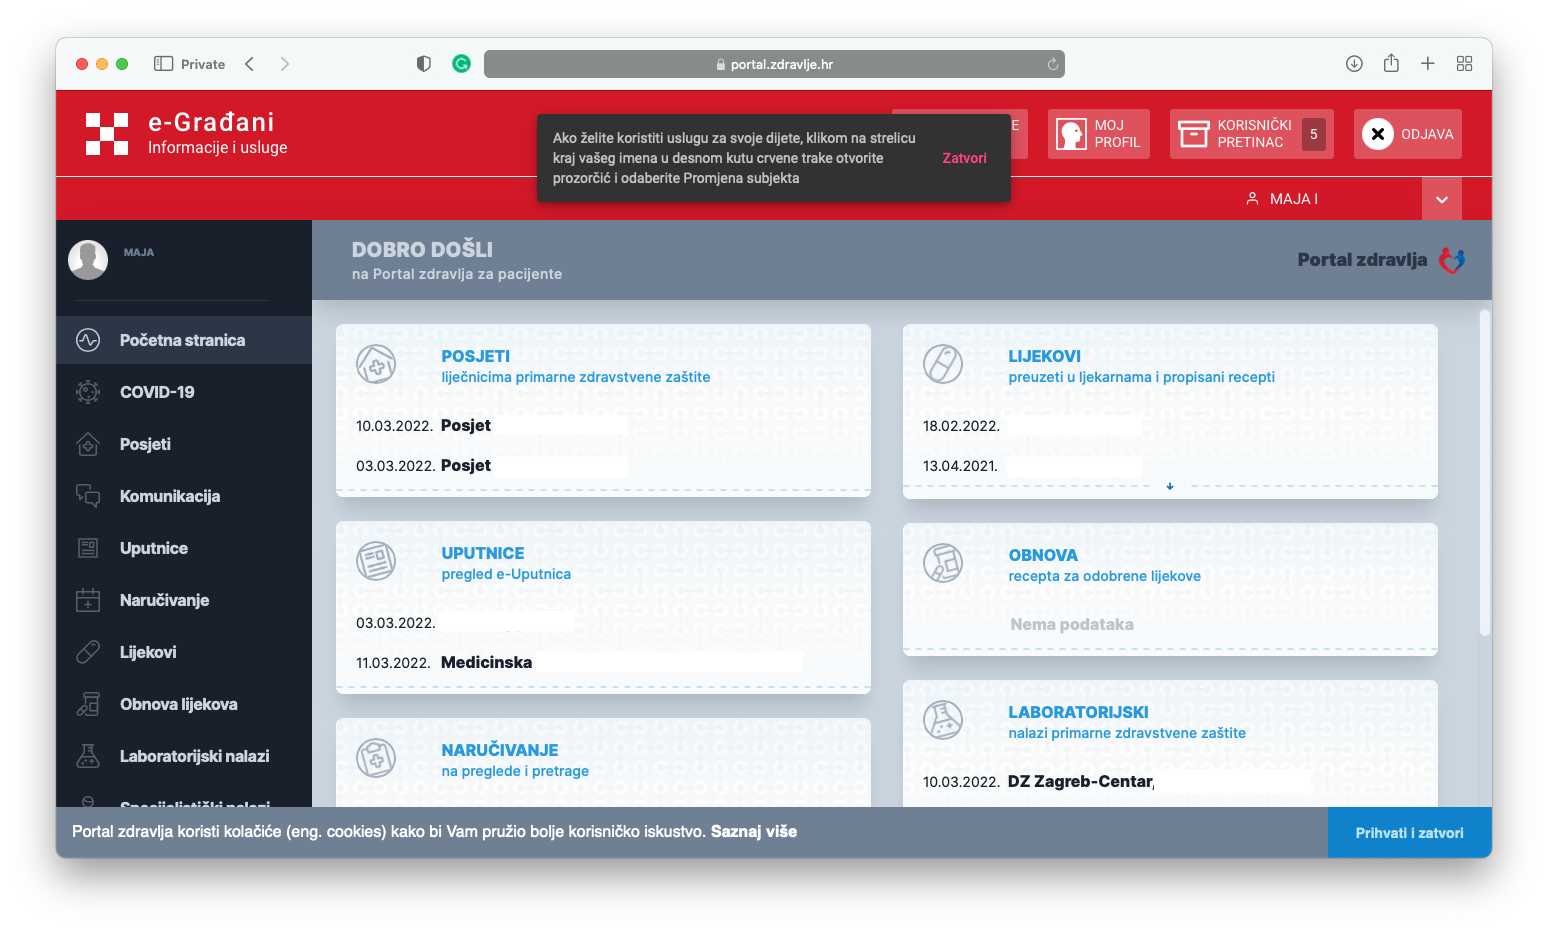
\includegraphics[width=\textwidth]{slike/portal_zdravlja.png} 
			\caption{Početna stranica "Portal zdravlje"}
			\label{fig:promjene2} 
\end{figure}
U konačnici, i "Ozdravi" i Portal zdravlja na e-Građani predstavljaju korisna digitalna rješenja za bolje upravljanje zdravstvenim informacijama, ali se razlikuju u svojoj svrsi, opsegu i ciljanoj publici. Oba projekta doprinose unaprjeđenju zdravstvene skrbi, svaki u svojem specifičnom kontekstu. \\
    
   Projekt "Ozdravi" je izveden kao web aplikacija, prilagođena različitim uređajima, uključujući mobilne uređaje, tablete i računalima. Osim toga, aplikacija je skalabilna i prilagodljiva za različite regije i zdravstvene ustanove.\\
    
    Opseg projektnog zadatka "Ozdravi" obuhvaća sve navedene funkcionalnosti i složenu koordinaciju između korisnika. Aplikacija omogućava brzu i preciznu komunikaciju između svih relevantnih strana. Kroz jednostavno i intuitivno sučelje, aplikacija omogućuje roditeljima, pedijatrima i liječnicima učinkovitije upravljanje zdravstvenim potrebama djece. \\
    
    Aplikacija pruža mogućnost za daljnji razvoj i proširenje, što će dodatno poboljšati iskustvo korisnika i olakšati njihovu svakodnevicu. Ova inovacija ima potencijal da unaprijedi kvalitetu života roditelja i omogući bolju skrb za djecu. Budući razvoj projekta "Ozdravi" može uključivati niz nadogradnji, uključujući integraciju s telemedicinom za daljinske konzultacije, razvoj mobilne aplikacija za veću dostupnost, proširenje podrške za različite jezike i regionalne prakse te poboljšanje analitičkih alata za praćenje medicinskih podataka. \\

	\eject
		
		
	
	\chapter{Specifikacija programske potpore}
		
	\section{Funkcionalni zahtjevi}
			
			\noindent \textbf{Dionici:}
			
			\begin{packed_enum}
				
				\item Roditelj
				\item Pedijatar
                \item Liječnik obiteljske medicine
                \item Administrator
                
			\end{packed_enum}
			
			\noindent \textbf{Aktori i njihovi funkcionalni zahtjevi:}
			
			
			\begin{packed_enum}
				\item  \underbar{Roditelj (inicijator) može:}
				
				\begin{packed_enum}
    
					\item registrirati se i prijaviti u sustav
                    \item vidjeti profil za sebe i svoju djecu
					\item pregledati medicinske nalaze, dijagnoze i povijesti pregleda za sebe i svoju djecu
                    \item zatražiti povratnu informaciju liječnika ili pedijatra o nalazu dobivenim temeljem određene usluge u privatnoj ustanovi, tj. drugog mišljenja
                    \item vidjeti druga mišljenja koja je stvorio
                    
				\end{packed_enum}
			
				\item  \underbar{Pedijatar (inicijator) može:}
				
				\begin{packed_enum}
			
					\item prijaviti se u sustav
                    \item prijaviti djecu po identifikatoru (OIB)
                    \item pregledati popis sve prijavljene djece i njihove kartone
					\item unijeti medicinske podatke (dijagnoze, preglede, terapije) i ažurirati te podatke
                    \item evidentirati preporuku za bolovanje za roditelja u slučaju bolesti djeteta
                    \item utvrditi bolest djeteta nakon čega se šalje ispričnica u školu ili vrtić
                    \item naručiti djecu na specijalističke preglede/postupke
                    \item dati povratnu informaciju na drugo mišljenje
                
				\end{packed_enum}

                \item  \underbar{Liječnik obiteljske medicine (inicijator) može:}
				
				\begin{packed_enum}
			
					\item prijaviti se u sustav
                    \item pregledati i odobriti doznake izdane od strane pedijatra koje se šalju poslodavcu roditelja
                    \item dati povratnu informaciju na drugo mišljenje
                    \item naručiti pacijenta na specijalistički pregled/postupak
                    \item unositi podatke o pregledima
                    \item pristupiti medicinskim nalazima, povijesti pregleda i upitima 
                    
				\end{packed_enum}
    
                \item  \underbar{Administrator (inicijator) može:}
				
				\begin{packed_enum}

                    \item prijava u sustav kao administrator
					\item pripremiti registre djece (osnovni podaci, OIB)
                    \item registrira liječnika obiteljske medicine i pedijatra
                    \item po registraciji roditelja, povezati iste s djecom (preko OIB-a)
					\item administrirati korisničke račune
                    \item ažurirati sve podatke u aplikaciji
                 
				\end{packed_enum}

                \item  \underbar{Baza podataka (sudionik):}
				
				\begin{packed_enum}

                    \item pohranjuje sve podatke o korisnicima i njihovim ovlastima
					
				\end{packed_enum}
    
			\end{packed_enum}
			
			\eject 
			
			
				
			\subsection{Obrasci uporabe}
				
				%dio 1. revizije
				
				\subsubsection{Opis obrazaca uporabe}
					%Funkcionalne zahtjeve razraditi u obliku obrazaca uporabe. Ukoliko u nekom koraku može doći do odstupanja, potrebno je to odstupanje opisati i po mogućnosti ponuditi rješenje kojim bi se tijek obrasca vratio na osnovni tijek.
					

					\noindent \underbar{\textbf{UC$<$broj obrasca$>$ -$<$ime obrasca$>$}}
					\begin{packed_item}
	
						\item \textbf{Glavni sudionik: }$<$sudionik$>$
						\item  \textbf{Cilj:} $<$cilj$>$
						\item  \textbf{Sudionici:} $<$sudionici$>$
						\item  \textbf{Preduvjet:} $<$preduvjet$>$
						\item  \textbf{Opis osnovnog tijeka:}
						
						\item[] \begin{packed_enum}
	
							\item $<$opis korak jedan$>$
							\item $<$opis korak dva$>$
							\item $<$opis korak tri$>$
							\item $<$opis korak četiri$>$
							\item $<$opis korak pet$>$
						\end{packed_enum}
						
						\item  \textbf{Opis mogućih odstupanja:}
						
						\item[] \begin{packed_item}
	
							\item[2.a] $<$opis mogućeg scenarija odstupanja u koraku 2$>$
							\item[] \begin{packed_enum}
								
								\item $<$opis rješenja mogućeg scenarija korak 1$>$
								\item $<$opis rješenja mogućeg scenarija korak 2$>$
								
							\end{packed_enum}
							\item[2.b] $<$opis mogućeg scenarija odstupanja u koraku 2$>$
							\item[3.a] $<$opis mogućeg scenarija odstupanja  u koraku 3$>$
							
						\end{packed_item}
					\end{packed_item}
				
					
				\subsubsection{Dijagrami obrazaca uporabe}
					
					%Prikazati odnos aktora i obrazaca uporabe odgovarajućim UML dijagramom. Nije nužno nacrtati sve na jednom dijagramu. Modelirati po razinama apstrakcije i skupovima srodnih funkcionalnosti.
				\eject		
				
			\subsection{Sekvencijski dijagrami}
				
				%dio 1. revizije
				
				%Nacrtati sekvencijske dijagrame koji modeliraju najvažnije dijelove sustava (max. 4 dijagrama). Uz svaki dijagram napisati detaljni opis dijagrama.
    
				\eject
	
		\section{Ostali zahtjevi}
		
			%dio 1. revizije
		 
			 %Nefunkcionalni zahtjevi i zahtjevi domene primjene dopunjuju funkcionalne zahtjeve. Oni opisuju kako se sustav treba ponašati i koja ograničenja treba poštivati (performanse, korisničko iskustvo, pouzdanost, standardi kvalitete, sigurnost...). Primjeri takvih zahtjeva u Vašem projektu mogu biti: podržani jezici korisničkog sučelja, vrijeme odziva, najveći mogući podržani broj korisnika, podržane web/mobilne platforme, razina zaštite (protokoli komunikacije, kriptiranje...)... Svaki takav zahtjev potrebno je navesti u jednoj ili dvije rečenice.
			 
			 
			 
	
	\chapter{Arhitektura i dizajn sustava}
		
		%dio 1. revizije

		Glavna tehnologija izrade "frontend" dijela sustava je React.js razvojni okvir, a samo korisničko sučelje je izgrađeno od gotovih komponenti iz paketa "Bootstrap". Korištenje Bootstrap-a nam omogućuje da brzo i lako razvijamo sučelja koja su izgledaju moderno i koja su responzivna, 
		što je jedan od važnijih zahtjeva. 

		Backend dio je izrađen u Spring radnom okviru koji omogućava razvoj MVC (Model-View-Controller) aplikacija, ali i još puno toga, poput rada s bazama podataka i autorizacije korisnika (Spring Security). 
		Za postavljanje aplikacije u skladu sa Springovim konvencijama koristili smo Spring Boot ekstenziju.

		Kao relacijsku bazu podataka odabrali smo Postgres. Radi se o bazi otvorenog koda \textit{(en. open-source)} visokih performansi koja se koristi za širok raspon zadataka i u raznim okruženjima.

		\begin{figure}[H]
			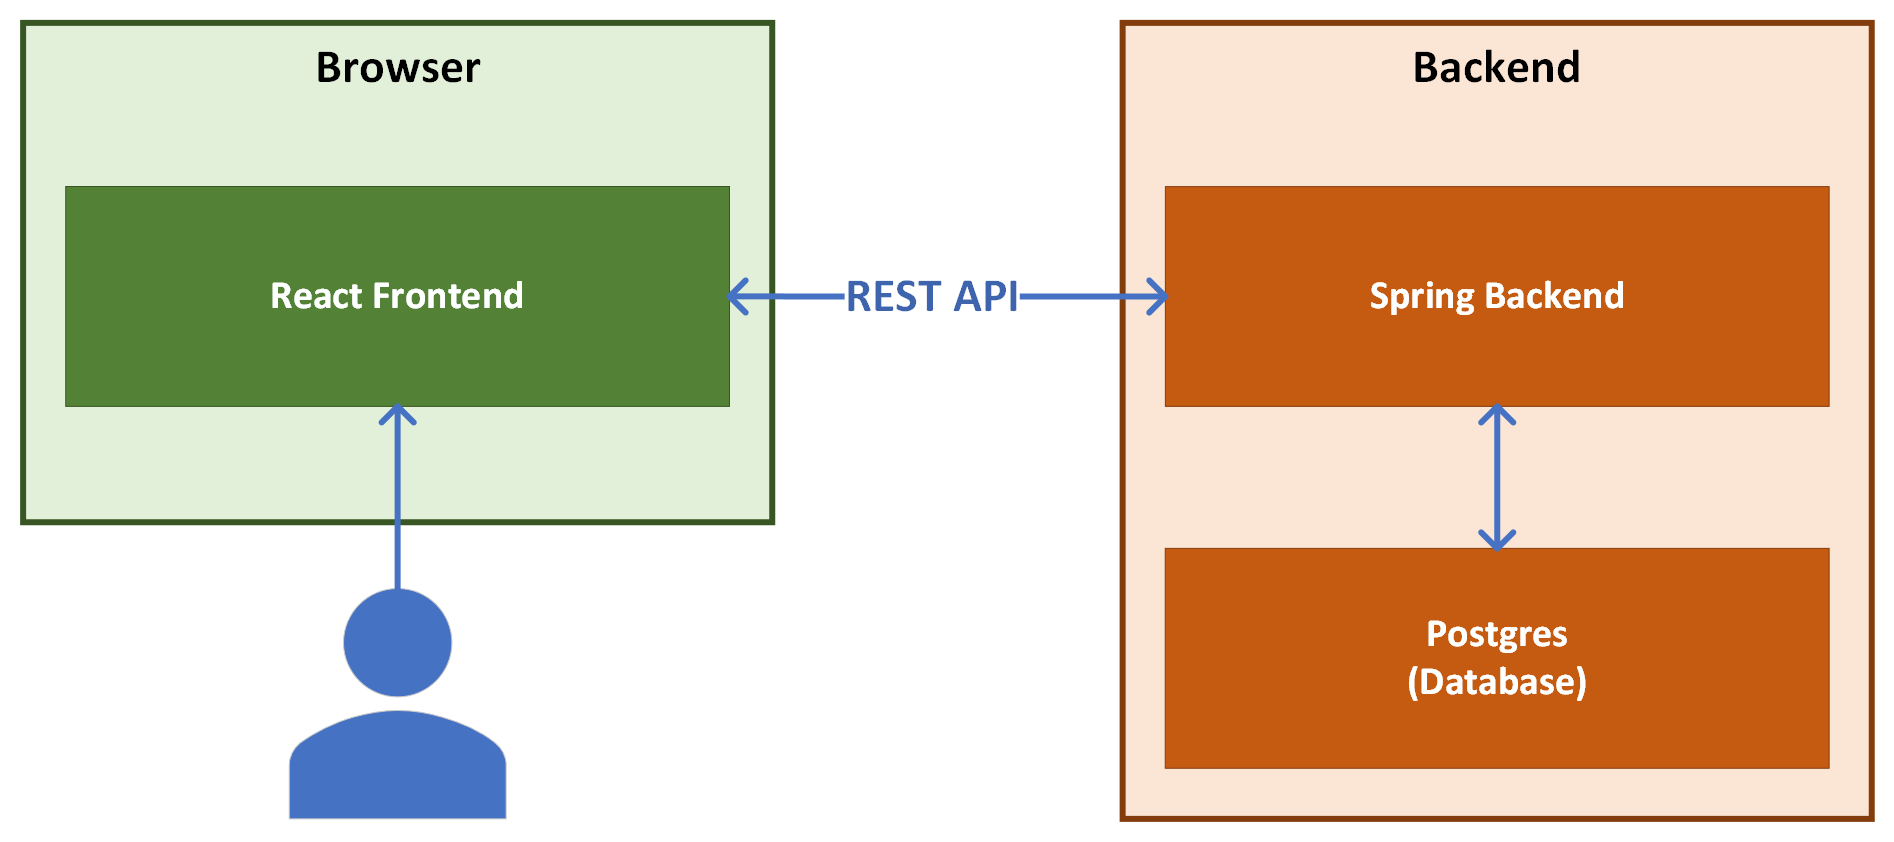
\includegraphics[width=\textwidth]{slike/architecture.png} 
			\caption{Dijagram arhitekture sustava "Ozdravi".}
			% \label{fig:promjene2} 
		\end{figure}

		Kao što je prikazano na slici 4.1, središnji je dio sustava Spring backend koji ostvaruje komunikaciju s Postgres bazom, ali i s frontend aplikacijom. Komunikacija s frontend-om se ostvaruje primjenom
		HTTP (HyperText Transfer Protokola) koji je ključni protokol web-a. Za potrebe komunikacije backend-a i frontend-a definiran je API (Application Programming Interface) u skladu s pravilima REST-a (Representational State Transfer). Neka od njih su:
		\begin{packed_item}
			\item odvajanje poslužitelja i klijenta - Klijent i poslužitelj su u potpunosti neovisni, a sve što klijent "zna" dolazi od poslužitelja.
			\item "statelessness" - 
		\end{packed_item}

		Važno je napomenuti da se React aplikacija izvršava unutar korisničkog preglednika, a ne na nekom vanjskom poslužitelju. Ipak, kako bi ju pokrenuo, korisnički preglednik tu aplikaciju mora preuzeti od negdje. To je oslikano u slici 4.2. 

		\begin{figure}[H]
			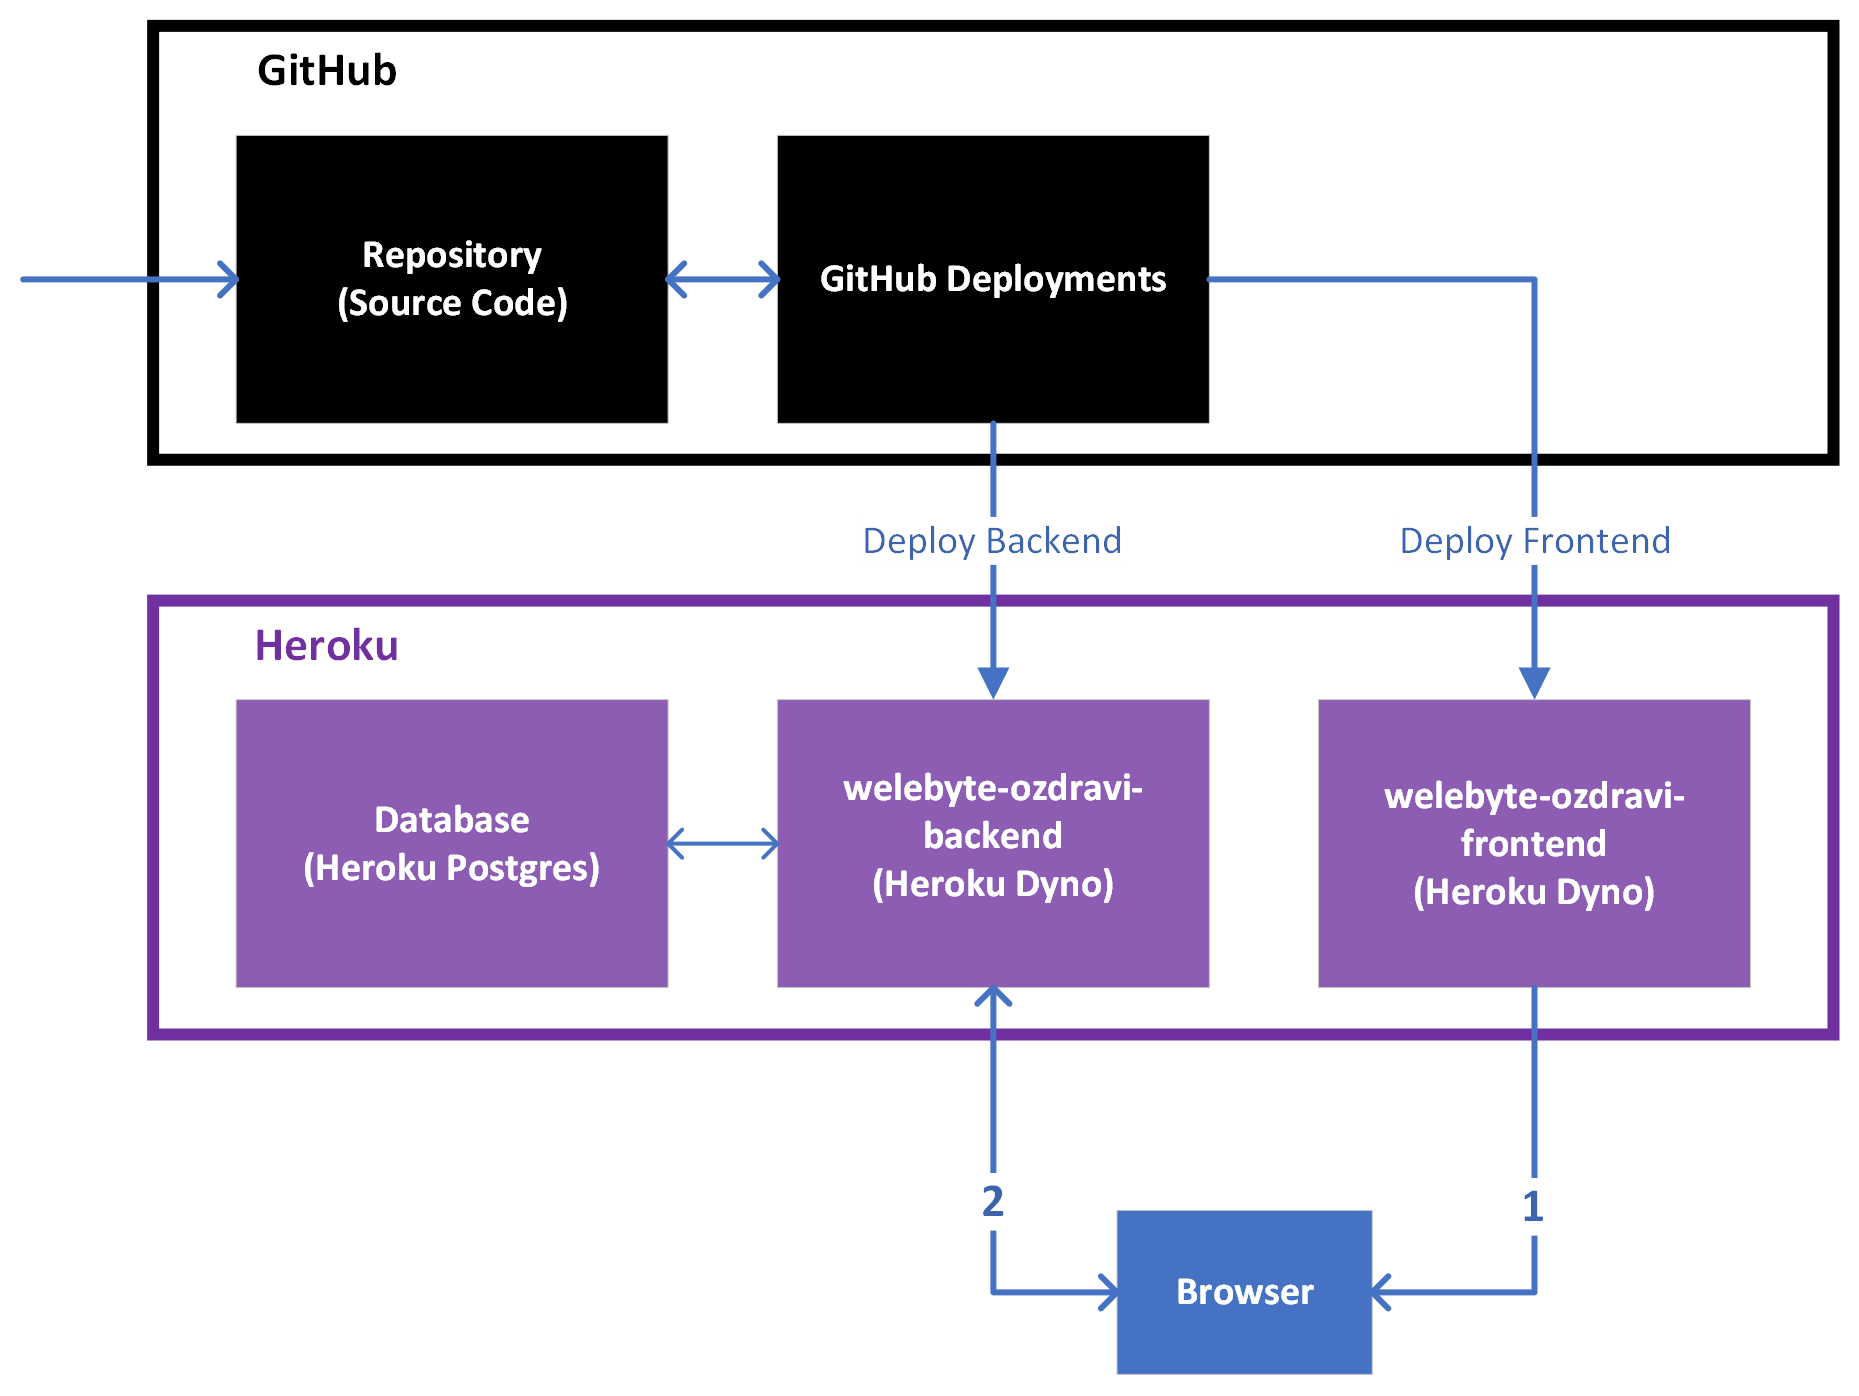
\includegraphics[width=\textwidth]{slike/infrastructure.png} 
			\caption{Dijagram infrastrukture sustava "Ozdravi".}
		\end{figure}

		U produkcijskom okruženju, sustav koristi dva poslužitelja - jedan pokreće Spring aplikaciju (backend), a drugi omogućava preglednicima preuzimanje React aplikacije (frontend).

		Kao infrastrukturnu platformu, na kojoj ćemo postaviti produkcijsko okruženje, izabrali smo Heroku iz dva glavna razloga:
		\begin{packed_item}
			\item jednostavnost postavljanja potrebnih resursa (Heroku Dyno, Heroku Postgres)
			\item fleksibilan model naplate koji omogućava da besplatno koristimo platformu
			\item jednostavno integriranje s GitHub repozitorijem za lak "deployment" kad je to potrebno
		\end{packed_item}
					
		\section{Baza podataka}
			
			%dio 1. revizije
			
		%Potrebno je opisati koju vrstu i implementaciju baze podataka ste odabrali, glavne komponente od kojih se sastoji i slično.
        Baza podataka koja se koristi u projektu "Ozdravi" ključna je komponenta sustava koja omogućava pohranu, upravljanje i praćenje svih relevantnih informacija o korisnicima i njihovim zdravstvenim podacima. Odabrana je relacijska baza podataka koja se sastoji od nekoliko ključnih entiteta:
            \begin{packed_item}
                \item Person
                \item Examination
                \item SecondOpinion
                \item Instruction
                \item SickLeaveRecommendation
                \item LoginCreds
            \end{packed_item}

        Baza podataka "Ozdravi" omogućava integraciju svih informacija kako bi podržala procese komunikacije, pregleda i dijagnoza u kontekstu brige o zdravstvenim potrebama djece. Ova struktura omogućava učinkovito praćenje i upravljanje svim relevantnim medicinskim podacima i podržava glavne funkcionalnosti sustava.
        
			\subsection{Opis tablica}

		\textbf{Osoba} Ovaj entitet sadržava osnovne informacije o svim korisnicima sustava. Sadrži atribute: identifikator osobe, identifikator roditelja osobe, identifikator pripadajućeg liječnika, identifikator adrese stanovanja osobe, OIB, ime, prezime, uloga u sustavu, lozinka te e-mail. Ovaj entitet je ključan za autentikaciju korisnika i definiranje njegove uloge unutar sustava.
		\begin{longtblr}[
			label=none,
			entry=none
			]{
				width = \textwidth,
				colspec={|X[6,l]|X[6, l]|X[20, l]|}, 
				rowhead = 1,
			} %definicija širine tablice, širine stupaca, poravnanje i broja redaka naslova tablice
			\hline \SetCell[c=3]{c}{\textbf{Person (osoba)}}	 \\ \hline[3pt]
			\SetCell{LightGreen}id & INT	&  	jedinstveni brojčani identifikator 	\\ \hline
			\SetCell{LightBlue}parent\_id	& INT & ID osobe koja je roditelj osobe [Parent] \\ \hline 
			\SetCell{LightBlue}doctor\_id	& INT & ID osobe koja je doktor osobe [Doctor/Pediatrician] \\ \hline 
			\SetCell{LightBlue}address\_id	& INT & ID Adrese osobe \\ \hline 
			OIB & VARCHAR & Osobni identifikacijski broj \\ \hline 
			first\_name & VARCHAR &  Ime osobe (NOT NULL) \\ \hline 
			last\_name & VARCHAR &  Prezime osobe (NOT NULL) \\ \hline 
			role & VARCHAR &  Uloga korisnika (NOT NULL) \\ \hline 
			password & VARCHAR &  Lozinka za prijavu u sustav \\ \hline
			email & VARCHAR &  e-mail za prijavu u sustav \\ \hline 
		\end{longtblr}

		\textbf{Pregled} Ovaj entitet sadržava podatke o pacijentima, uključujući informacije o njihovim pregledima, dijagnozama i zapisnicima. Sadrži atribute: identifikator pregleda, identifikator pacijenta, identifikator liječnika, identifikator liječnika koji je zakazao pregled, identifikator adrese na kojoj se održava pregled, zapisnik s pregleda te datum i vrijeme pregleda. Pohranjuje veze između pacijenata, doktora i pregleda, omogućavajući praćenje medicinskih podataka. 
		
		\begin{longtblr}[
			label=none,
			entry=none
			]{
				width = \textwidth,
				colspec={|X[6,l]|X[6, l]|X[20, l]|}, 
				rowhead = 1,
			} 
			\hline \SetCell[c=3]{c}{\textbf{Examination (Pregled)}}	 \\ \hline[3pt]
			\SetCell{LightGreen}id & INT	&  	jedinstveni brojčani identifikator 	\\ \hline
			\SetCell{LightBlue}patient\_id	& INT & ID osobe koja je pacijent [Parent/Child] (NOT NULL) \\ \hline 
			\SetCell{LightBlue}doctor\_id	& INT & ID osobe koja vrši pregled [Doctor/Pediatrician] (NOT NULL) \\ \hline 
			\SetCell{LightBlue}scheduler\_id	& INT & ID osobe koja je zakazala pregled [Doctor/Pediatriciran] (NOT NULL) \\ \hline 
			\SetCell{LightBlue}address\_id	& INT & ID adrese na kojoj se održava pregled \\ \hline 
			report & TEXT & Dijagnoza/zapisnik s pregleda \\ \hline 
			date & DATETIME &  Datum i vrijeme pregleda (NOT NULL) \\ \hline 
		\end{longtblr}

		\textbf{Drugo mišljenje} Ovaj entitet služi za praćenje detalja o pregledima pacijenata. Sadrži atribute: identifikator drugog mišljenja, identifikator osobe koja ga je zatražila, identifikator liječnika koji daje drugo mišljenje te nalaz iz privatne ustanove na temelju kojeg se traži drugo mišljenje. Ovaj entitet omogućava praćenje medicinskih konzultacija.
		\begin{longtblr}[
			label=none,
			entry=none
			]{
				width = \textwidth,
				colspec={|X[6,l]|X[6, l]|X[20, l]|}, 
				rowhead = 1,
			} 
			\hline \SetCell[c=3]{c}{\textbf{SecondOpinion (DrugoMišljenje)}}	 \\ \hline[3pt]
			\SetCell{LightGreen}id & INT	&  	jedinstveni brojčani identifikator 	\\ \hline
			\SetCell{LightBlue}requester\_id	& INT & ID osobe koja je zatražila drugo mišljenje [Parent] (NOT NULL) \\ \hline 
			\SetCell{LightBlue}doctor\_id & INT & ID osobe koja je dala drugo mišljenje [Doctor/Pediatrician] (NOT NULL) \\ \hline 
			private\_report & TEXT & nalaz iz privatne ustanove koji unosi roditelj (NOT NULL)\\ \hline 
			content & TEXT &  Sadržaj na koji se daje drugo mišljenje (nalaz iz privatne ustanove) \\ \hline 
		\end{longtblr}

		\textbf{Uputa} Ovaj entitet sadržava informacije o izdanim uputama, uključujući informacije o pacijentima, doktorima koji stvaraju upute i statusu upute. Sadrži atribute: identifikator upute, identifikator liječnika koji je izdao uputu, identifikator pacijenta kojemu je upućena, identifikator adrese, datum te sadržaj upute. Omogućava praćenje i upravljanje medicinskim preporukama.
		\begin{longtblr}[
			label=none,
			entry=none
			]{
				width = \textwidth,
				colspec={|X[6,l]|X[6, l]|X[20, l]|}, 
				rowhead = 1,
			} 
			\hline \SetCell[c=3]{c}{\textbf{Instruction (Uputa)}}	 \\ \hline[3pt]
			\SetCell{LightGreen}id & INT	&  	jedinstveni brojčani identifikator 	\\ \hline
			\SetCell{LightBlue}doctor\_id	& INT & ID osobe koja je izdala uputu [Doctor/Pediatrician] (NOT NULL) \\ \hline 
			\SetCell{LightBlue}patient\_id & INT & ID osobe za koju je uputa [Parent] (NOT NULL) \\ \hline 
            \SetCell{LightBlue}address\_id	& INT & ID adrese na kojoj će se održati pregled za danu uputu (NOT NULL) \\ \hline 
			date & DATETIME & Datum i vrijeme izdavanja upute (NOT NULL)\\ \hline 
			content & TEXT &  Sadržaj upute (NOT NULL) \\ \hline 
		\end{longtblr}

		\textbf{Preopurka za bolovanje} Ovaj entitet sadržava informacije o izdanim preporukama za bolovanje, tko ih je izdao, za koga i tko ih treba odobriti. Sadrži atribute: identifikator preporuke, identifikator pacijenta, identifikator pedijatra koji ju je stvorio, identifikatora liječnika koji ju je odobrio, identifikator pregleda na kojem se izdaje, e-mail adresa posolodavca kojem se šalje doznaka za bolovanje te status preporuke.
		\begin{longtblr}[
			label=none,
			entry=none
			]{
				width = \textwidth,
				colspec={|X[6,l]|X[6, l]|X[20, l]|}, 
				rowhead = 1,
			} 
			\hline \SetCell[c=3]{c}{\textbf{SickLeaveRecommendation (Preporuka za bolovanje)}}	 \\ \hline[3pt]
			\SetCell{LightGreen}id & INT	&  	jedinstveni brojčani identifikator	\\ \hline
			\SetCell{LightBlue}patient\_id & INT & ID osobe za koju se traži bolovanje [Parent] (NOT NULL) \\ \hline 
			\SetCell{LightBlue}creator\_id & INT & ID osobe koja je stvorila preporuku [Pediatrician] (NOT NULL) \\ \hline
			\SetCell{LightBlue}approver\_id & INT & ID osobe koja mora odobriti preporuku [Doctor] (NOT NULL) \\ \hline 
			\SetCell{LightBlue}examination\_id	& INT & ID pregleda na temelju kojeg se izdaje preporuka (NOT NULL) \\ \hline 
			email & VARCHAR & e-mail poslodavca na koji se šalje doznaka, ako je potvrđena preporuka(NOT NULL) \\ \hline 
			status & BOOLEAN &  Je li preporuka odobrena? (default false) \\ \hline 
		\end{longtblr}

        \textbf{Adresa} Ovaj entitet sadržava informacije o adresi održavanja pregleda. Sadrži atribute: identifikator ulice, ulicu, kućni broj, grad, državu te geografsku širinu i dužinu. 
		\begin{longtblr}[
			label=none,
			entry=none
			]{
				width = \textwidth,
				colspec={|X[6,l]|X[6, l]|X[20, l]|}, 
				rowhead = 1,
			} 
			\hline \SetCell[c=3]{c}{\textbf{Address (Adresa)}}	 \\ \hline[3pt]
			\SetCell{LightGreen}id & INT	&  	jedinstveni brojčani identifikator 	\\ \hline
			street	& VARCHAR & ulica\\ \hline 
            number	& VARCHAR & kućni broj\\ \hline
            city	& VARCHAR & grad\\ \hline
            country	& VARCHAR & država\\ \hline
            latitude	& NUMERIC & geografska širina\\ \hline
            longitude	& NUMERIC & geografska dužina\\ \hline
			
		\end{longtblr}
  
		\subsection{Dijagram baze podataka}
			% U ovom potpoglavlju potrebno je umetnuti dijagram baze podataka. Primarni i strani ključevi moraju biti označeni, a tablice povezane. Bazu podataka je potrebno normalizirati.
		    \begin{figure}[H]
			     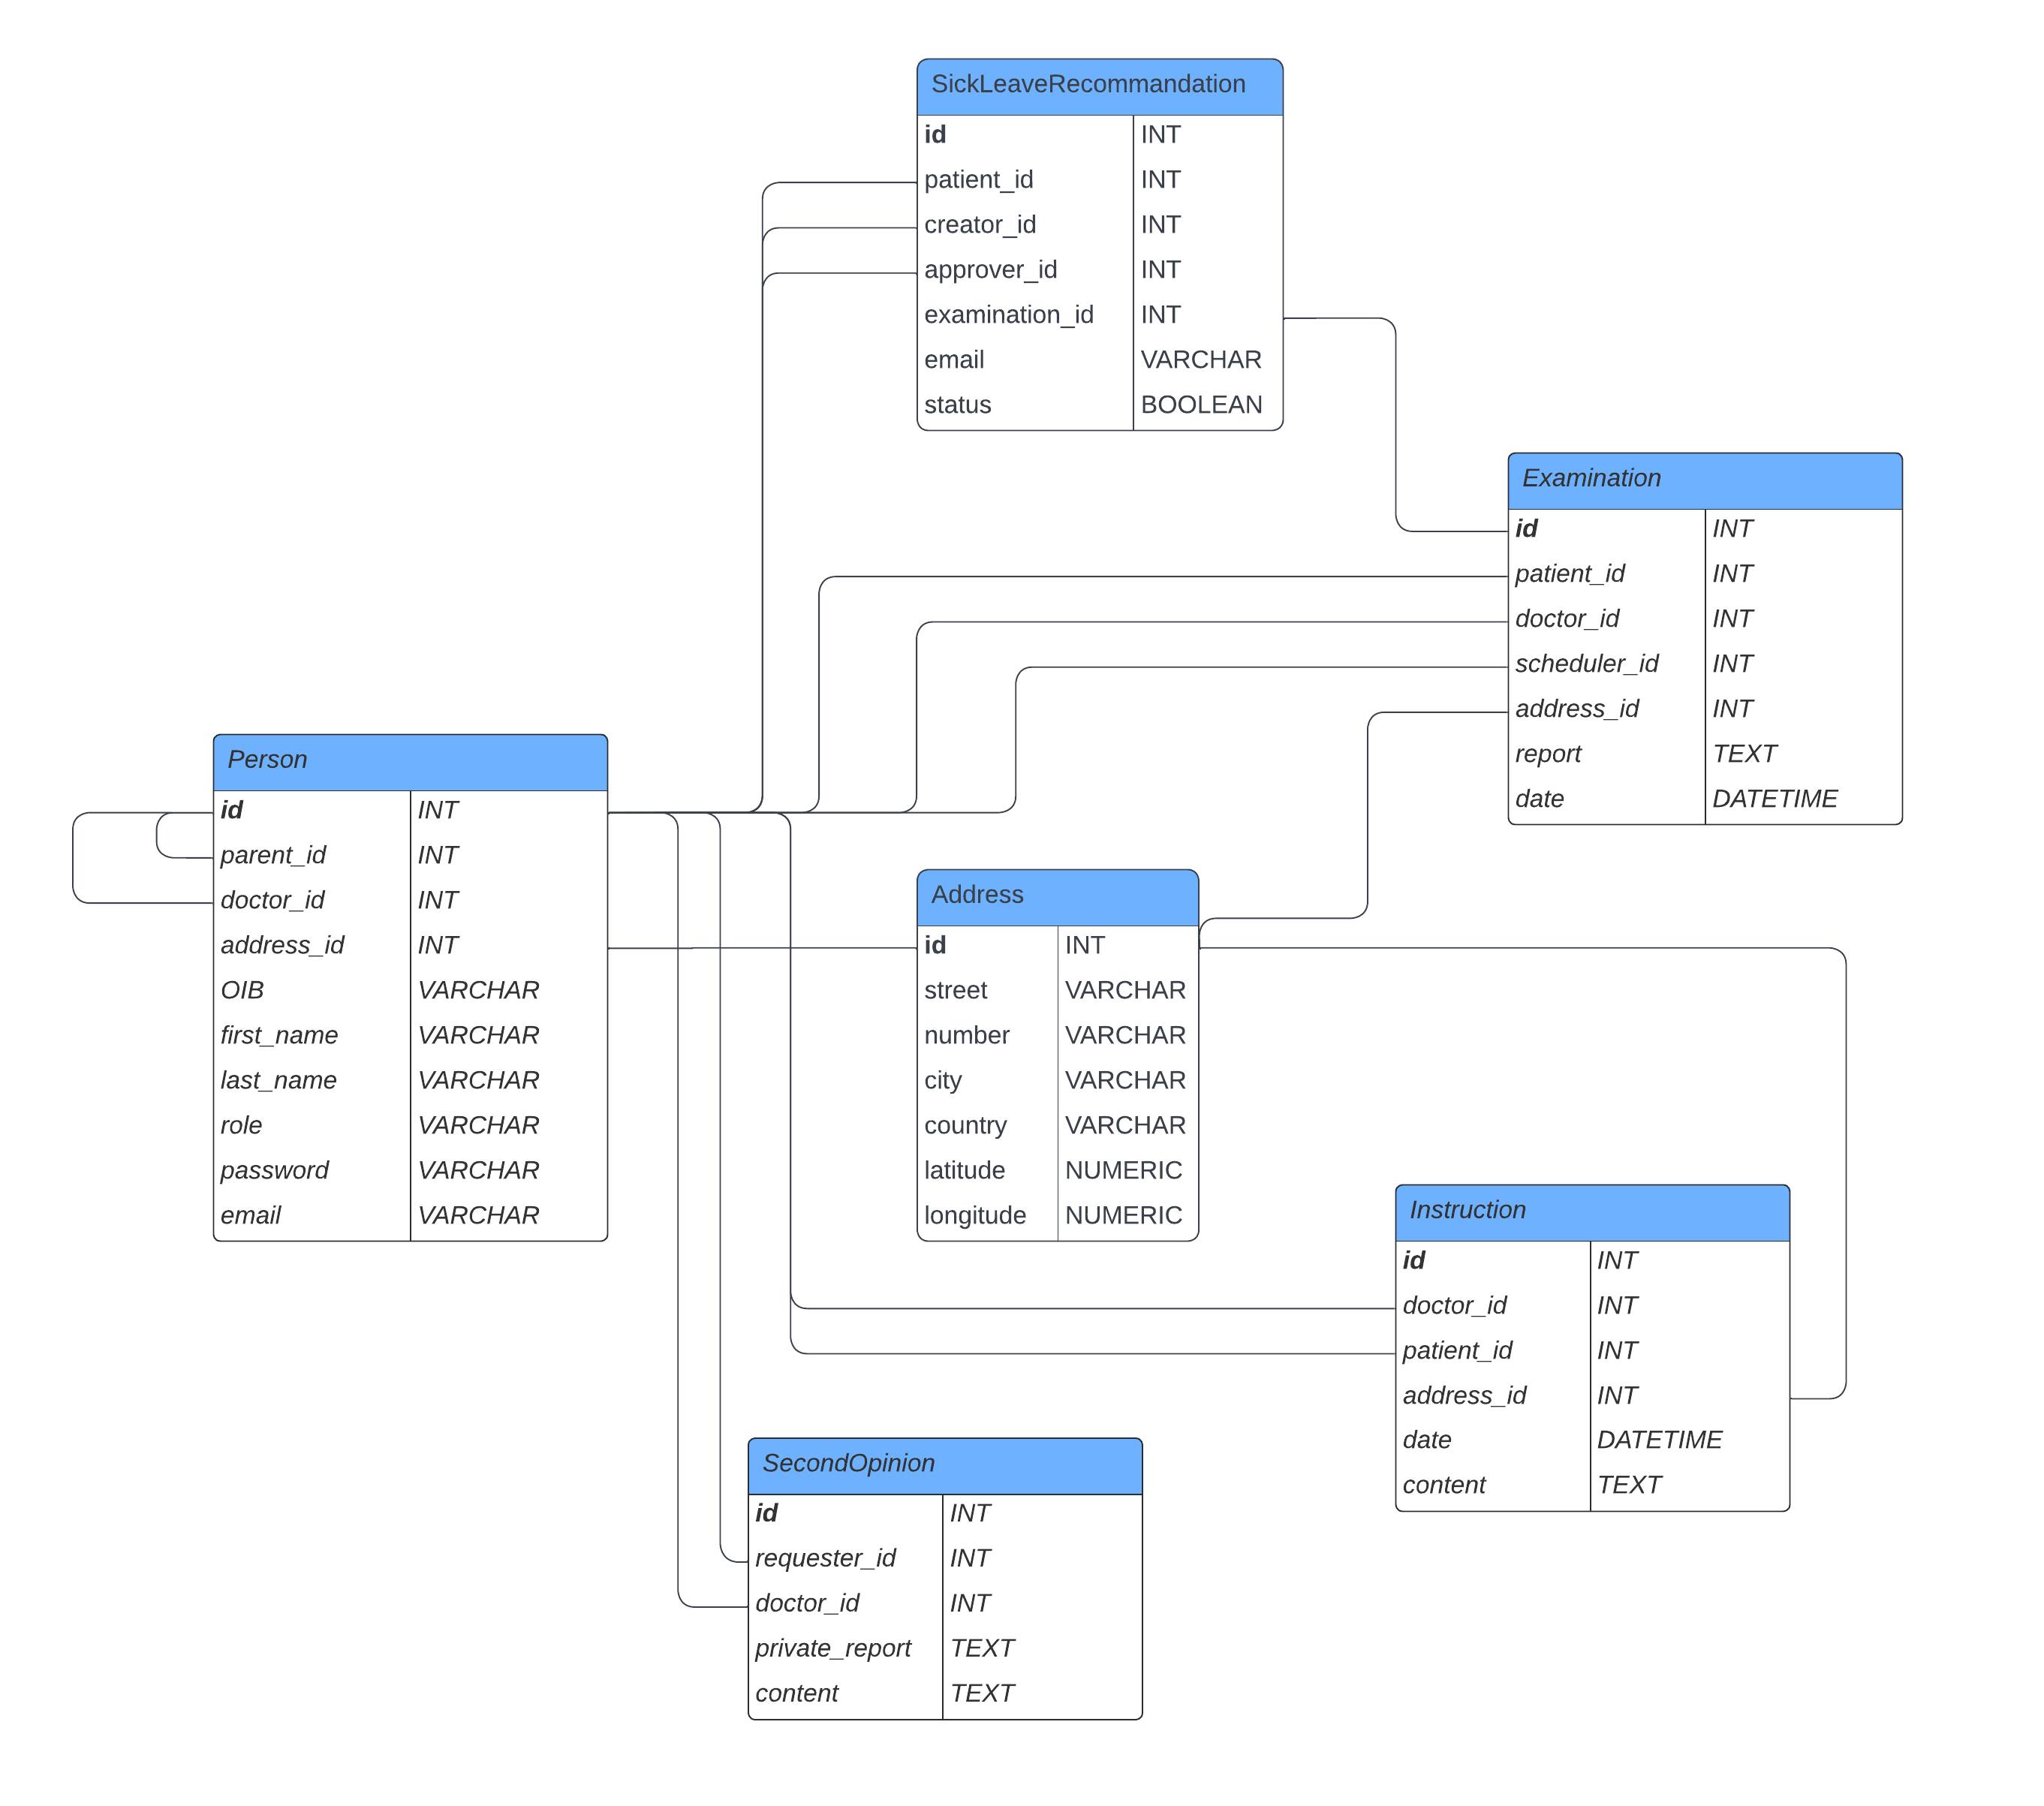
\includegraphics[width=\textwidth]{dokumentacija/slike/ERdijagram.png} 
			     \caption{ER dijagram baze podataka} 
		    \end{figure}
		\eject
		
			
		\section{Dijagram razreda}
		
			%Potrebno je priložiti dijagram razreda s pripadajućim opisom. Zbog preglednosti je moguće dijagram razlomiti na više njih, ali moraju biti grupirani prema sličnim razinama apstrakcije i srodnim funkcionalnostima.
			
			%dio 1. revizije
			
			%Prilikom prve predaje projekta, potrebno je priložiti potpuno razrađen dijagram razreda vezan uz generičku funkcionalnost sustava. Ostale funkcionalnosti trebaju biti idejno razrađene u dijagramu sa sljedećim komponentama: nazivi razreda, nazivi metoda i vrste pristupa metodama (npr. javni, zaštićeni), nazivi atributa razreda, veze i odnosi između razreda.
			
			%dio 2. revizije			
			
			%Prilikom druge predaje projekta dijagram razreda i opisi moraju odgovarati stvarnom stanju implementacije
			
			
			
			\eject
		
		\section{Dijagram stanja}
			
			
			%dio 2. revizije
			
			%Potrebno je priložiti dijagram stanja i opisati ga. Dovoljan je jedan dijagram stanja koji prikazuje značajan dio funkcionalnosti sustava. Na primjer, stanja korisničkog sučelja i tijek korištenja neke ključne funkcionalnosti jesu značajan dio sustava, a registracija i prijava nisu.
			
			
			\eject 
		
		\section{Dijagram aktivnosti}
			
			%dio 2. revizije
			
			 %Potrebno je priložiti dijagram aktivnosti s pripadajućim opisom. Dijagram aktivnosti treba prikazivati značajan dio sustava.
			
			\eject
		\section{Dijagram komponenti}
		
			%dio 2. revizije
		
			 %Potrebno je priložiti dijagram komponenti s pripadajućim opisom. Dijagram komponenti treba prikazivati strukturu cijele aplikacije.
	\chapter{Implementacija i korisničko sučelje}
		\section{Korištene tehnologije i alati}		
			 U tijeku razvoja projekta "Ozdravi", pažljivo su odabrane i implementirane različite tehnologije i alati kako bi se postigla efikasna izrada dokumentacije i aplikacije za zdravstveni sustav.
			 Za unapređenje timskih komunikacija korištene su aplikacije \textit{WhatsApp}\footnote{\url{https://www.whatsapp.com}} i \textit{Microsoft Teams}\footnote{\url{https://www.microsoft.com/en-us/microsoft-teams/group-chat-software}}. WhatsApp, popularna platforma za brzu razmjenu poruka, olakšala je neposrednu interakciju među članovima tima, dok je Microsoft Teams pružio šire mogućnosti za suradnju, uključujući organizaciju sastanaka, održavanje sastanaka i dijeljenje datoteka.
			 U praćenju zadataka i upravljanju projektom koristila se \textit{Jira}\footnote{\url{https://www.atlassian.com/software/jira}}, snažan alat koji je omogućio stvaranje strukturirane i pregledne radne okoline. Jira je poslužila kao središnje mjesto za praćenje i planiranje aktivnosti, olakšavajući koordinaciju među članovima tima.
			 \textit{GitHub}\footnote{\url{https://github.com}} se istaknuo kao ključni alat za upravljanje izvornim kodom i omogućavanje učinkovite suradnje među članovima tima. GitHub, kao web-bazirana platforma, pružio je mogućnost distribuiranog upravljanja verzijama korištenjem Git sustava. Repozitorij na GitHubu služio je kao centralno mjesto za čitav izvorni kod, omogućavajući članovima tima sinkroniziranje svojih lokalnih kopija koda, praćenje promjena te učinkovito upravljanje raznim granama razvoja.
			 \textit{Astah}\footnote{\url{http://astah.net/editions/professional}} je korišten za izradu UML dijagrama, pružajući jasan prikaz strukture sustava i odnosa između njegovih dijelova. Osim Astaha, korišteni su i drugi alati za izradu dijagrama, uključujući \textit{Visual Paradigm}\footnote{\url{https://online.visual-paradigm.com}} i \textit{Lucidchart}\footnote{\url{https://www.lucidchart.com}}.
			 Za razvoj frontend dijela aplikacije korišten je \textit{React}\footnote{\url{https://reactjs.org/}}, jedna od najpopularnijih \textit{JavaScript}\footnote{\url{https://www.javascript.com/}} biblioteka koja omogućava dinamičko i responzivno korisničko sučelje. React je pridonosio brzoj izgradnji modernog sučelja s visokom interaktivnošću.
			 Korišten je i \textit{Bootstrap}\footnote{\url{https://getbootstrap.com}}, popularni okvir za izradu responzivnih web stranica, koji je omogućio brzo i jednostavno oblikovanje sučelja te moderan i funkcionalan dizajn. Bootstrap pruža jednostavne i učinkovite klase za organizaciju elemenata, responzivno oblikovanje pomoću tzv. grid sustava te unaprijed definirane stilove za tipografiju, forme, gumbiće i mnoge druge komponente.
			 Za backend je odabran \textit{Spring}\footnote{\url{https://spring.io}}, robustan okvir za razvoj \textit{Java}\footnote{\url{https://www.java.com/en/}} aplikacija. Spring je pružio strukturu i podršku za izradu pouzdanih, sigurnih i skalabilnih backend rješenja.
			 API sustav je strukturiran i dokumentiran korištenjem alata \textit{Swagger}\footnote{\url{https://swagger.io}}, pri čemu je implementiran sukladno OpenAPI konvencijama. OpenAPI pristup omogućava jednostavno definiranje, dokumentiranje i testiranje RESTful API-ja te definiranje svih dostupnih endpointa, parametara, odgovora i modela podataka.
			 U procesu pisanja koda korišteni su \textit{IntelliJ IDEA}\footnote{\url{https://www.jetbrains.com/idea/}} i \textit{Visual Studio Code}\footnote{\url{https://visualstudio.microsoft.com/}}. IntelliJ IDEA, s bogatim skupom značajki, podržavao je razvoj Java aplikacija, dok je Visual Studio Code, lagan i svestran, omogućavao efikasno pisanje koda u različitim jezicima, uključujući \textit{JavaScript}\footnote{\url{https://www.javascript.com/}}.
			 Odabir ovih alata bio je prepušten osobnim preferncijama članova tima.
			 Za postavljanje produkcijskog okruženja odabran je Heroku kao infrastrukturna platforma. \textit{Heroku}\footnote{\url{https://www.heroku.com}} pruža stabilnost i skalabilnost, čineći implementaciju i održavanje aplikacije jednostavnim i učinkovitim.
			 Baza podataka \textit{PostgreSQL}\footnote{\url{https://www.postgresql.org}} koristila se za trajno pohranjivanje podataka. PostgreSQL je open-source sustav za upravljanje bazama podataka koji pruža pouzdano i sigurno okruženje za pohranu informacija.
			 U konačnici, ovom kombinacijom tehnologija postignuto je stvaranje moderne zdravstvene aplikacije koja je intuitivna za korisnike, prilagodljiva potrebama zdravstvenog sustava i unapređuje ukupno iskustvo krajnjih korisnika.
			\eject 
	
		\section{Ispitivanje programskog rješenja}
			Ispitivanje programskog rješenja predstavlja ključan korak u procesu razvoja programske podrške s ciljem ostvarivanja nekoliko ključnih prednosti:
			\begin{packed_item}
				\item olakšava dodavanje značajki - ispitivanje osigurava da nove promjene ne nraušavaju funkcionalnost postojećeg koda
				\item sprječava unošenje grešaka u kod - kvalitetni testovi detektiraju neispravan kod prije nego što postane dio projekta čime se smanjuje mogućnost pojave grešaka
			\end{packed_item}
			
			U sklopu ovog projekta koristili smo dvije vrste ispitivanja:
			\begin{packed_item}
				\item Ispitivanje komponenti (eng. Unit Testing)
				\item Ispitivanje sustava (eng. Integration Testing)
			\end{packed_item}
			
			
			Ispitivanjem komponenti koristeći JUnit biblioteke osigurali smo ispravan rad ključnih dijelovi backenda. Ispitivanjem sustava provjerili smo ispravnost povezanosti backenda i frontenda iz perspektive krajnjeg korisnika.
			Ispitivanje sustava je provedeno koristeći Selenium biblioteke.
			
			%==========================================================================================================================%
			\subsection{Ispitivanje komponenti}
			\subsubsection*{Test 1: Ispitivanje ispravnog OIB-a}
			Komponenta: ValidityUtil \newline
			Metoda: public static boolean isValidOib(String oib); \newline
			Ulazni Podaci: 
			\begin{packed_item}
				\item String oib : "39751670659"
			\end{packed_item}
			Očekivani rezultat:
			\begin{packed_item}
				\item Metoda vraća istinu (true) jer je OIB ispravan prema standardu za OIB-e.
			\end{packed_item}
			\lstinputlisting[style=JavaStyle, caption={Test 1}]{code/oib_test_1.java}

			\subsubsection*{Test 2: Ispitivanje neispravnog OIB-a}
			Komponenta: ValidityUtil \newline
			Metoda: public static boolean isValidOib(String oib); \newline
			Ulazni Podaci: 
			\begin{packed_item}
				\item String oib : "397516706.9"
			\end{packed_item}
			Očekivani rezultat:
			\begin{packed_item}
				\item Metoda vraća laž (false) jer OIB sadrži '.', odnosno ne zadovoljava standardni oblik.
			\end{packed_item}
			\lstinputlisting[style=JavaStyle, caption={Test 2}]{code/oib_test_2.java}

			U testovima namijenjenima testiranju kontrolera, želimo ispitati isključivo ponašanje kontrolera, bez ispitivanja servisa, baze i drugih dijelova aplikacije.
			Budući da kontoleri ne mogu raditi bez tih dijelova, nužno je stvoriti "mock" objekte koji ih mijenjaju i simuliraju njihovo ponašanje.

			Ovaj postupak uključuje ručno stvaranje entiteta koji predstavljaju očekivane rezultate servisa.

			\subsubsection*{Test 3: Dohvaćanje popisa Uputa.}
			Komponenta: InstructionsController \newline
			Zahtjev: HTTP GET /instructions \newline
			Mock Podaci:
			\begin{packed_item}
				\item Korisnik
				\item Pregledi kojima korisnik može pristupiti
			\end{packed_item}
			Očekivani rezultat:
			\begin{packed_item}
				\item Kontroler u JSON formatu vraća popis svih Uputa koje trenutni korisnik može vidjeti, HTTP odgovor ima status 201 (OK).
			\end{packed_item}
			\lstinputlisting[style=JavaStyle, caption={Test 3}]{code/instruction_test_1.java}
			
			\subsubsection*{Test 4: Stvaranje Uputa.}
			Komponenta: InstructionsController \newline
			Zahtjev: HTTP POST /instructions \newline
			Mock Podaci:
			\begin{packed_item}
				\item Korisnik (ADMIN)
			\end{packed_item}
			Očekivani rezultat:
			\begin{packed_item}
				\item Kontroler u JSON formatu vraća atribute novostvorene Upute, HTTP odgovor ima status 201 (Created).
			\end{packed_item}
			\lstinputlisting[style=JavaStyle, caption={Test 4}]{code/instruction_test_2.java}

			\subsubsection*{Test 5: Dohvaćanje nepostojeće Upute.}
			Komponenta: InstructionsController \newline
			Zahtjev: HTTP GET /instruction/\{id\} \newline
			Mock Podaci:
			\begin{packed_item}
				\item Korisnik (ADMIN)
			\end{packed_item}
			Očekivani rezultat:
			\begin{packed_item}
				\item HTTP odgovor ima status 404 (Not Found).
			\end{packed_item}
			\lstinputlisting[style=JavaStyle, caption={Test 5}]{code/instruction_test_3.java}

			\subsubsection*{Test 6: Dohvaćanje svih doktora u aplikaciji.}
			Komponenta: UsersController \newline
			Zahtjev: HTTP GET /users/doctors \newline
			Mock Podaci:
			\begin{packed_item}
				\item Korisnik (PARENT)
			\end{packed_item}
			Očekivani rezultat:
			\begin{packed_item}
				\item HTTP odgovor ima status 403 (Forbidden), jer roditelj ne smije dobiti popis svih liječnika u aplikciji.
			\end{packed_item}
			\lstinputlisting[style=JavaStyle, caption={Test 6}]{code/user_test_1.java}
			
			\subsubsection*{Test 7: Dodavanje korisnika.}
			Komponenta: UsersController \newline
			Zahtjev: HTTP POST /users \newline
			Mock Podaci:
			\begin{packed_item}
				\item Korisnik (ADMIN)
			\end{packed_item}
			Očekivani rezultat:
			\begin{packed_item}
				\item Kontroler u JSON formatu vraća atribute novostvorenog Korisnika, HTTP odgovor ima status 201 (Created).
			\end{packed_item}
			\lstinputlisting[style=JavaStyle, caption={Test 7}]{code/user_test_2.java}

			\subsubsection*{Test 8: Registracija korisnika.}
			Komponenta: AuthenticationController \newline
			Zahtjev: HTTP POST /register \newline
			Očekivani rezultat:
			\begin{packed_item}
				\item Kontroler u JSON formatu vraća atribute novostvorenog Korisnika, HTTP odgovor ima status 201 (Created).
			\end{packed_item}
			\lstinputlisting[style=JavaStyle, caption={Test 8}]{code/registration_test.java}

			\begin{figure}[H]
				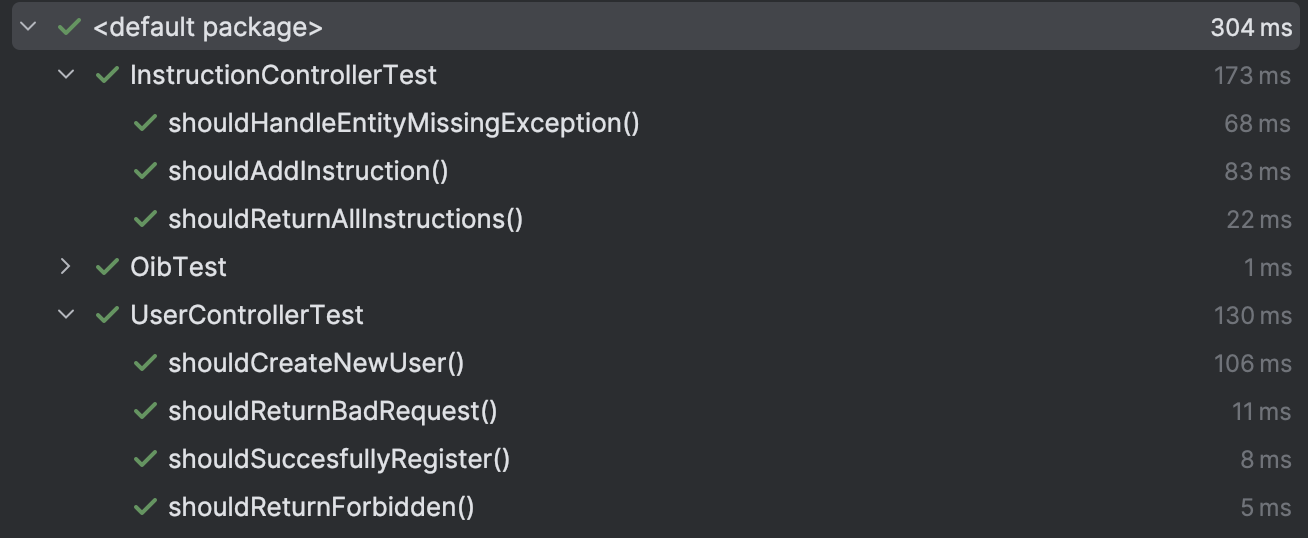
\includegraphics[width=\textwidth]{slike/testing_results.png} 
				\caption{Rezultati testiranja na lokalnom stroju.} 
			\end{figure}
			
			%==========================================================================================================================%
			\subsection{Ispitivanje sustava}
			Testovi ispitivanja sustava su napisani u Selenium IDE dodatku za preglednik i prate nekoliko obrazaca uporabe, ali su vezani uz jednu cjelinu - rad s preporukama za bolovanje.
			U ovom scenariju testiranja sudjeluje više uloga (roditelj, pedijatar, liječnik) i svi koraci koje jedna uloga izvodi su grupirani u zasebnu "grupu koraka". Također, za svaki korak je
			naveden i pripadajući očekivani rezultat.
			
			 \subsubsection*{Grupa koraka 1: Dodavanje preporuke za bolovanje}
			 Koraci:
			 \begin{packed_enum}
				\item Prijava u sustav kao pedijatar ("pedijatar@mail.com")
				\item Odabir opcije "Bolovanja" iz alatne trake.
				\item Odabir opcije "Dodaj preporuku"
				\item Odabir pregleda na temelju kojeg se izdaje preporuka ("Tamara Stanic 2023-12-25") unutar modalnog ekrana.
				\item Odabir opcije "Spremi".
			 \end{packed_enum}
			 Očekivani rezultati:
			 \begin{packed_enum}
				\item Pedijatar se može prijaviti u sustav.
				\item Postoji opcija "Bolovanja" u alatnoj traci.
				\item Dostupna je opcija "Dodaj preporuku".
				\item Postoji izbornik pregleda unutar modalnog ekrana u kojem je moguće izabrati traženi pregled.
				\item Postoji opcija "Spremi" unutar modalnog ekrana.
			 \end{packed_enum}
			 
			 \begin{figure}[H]
				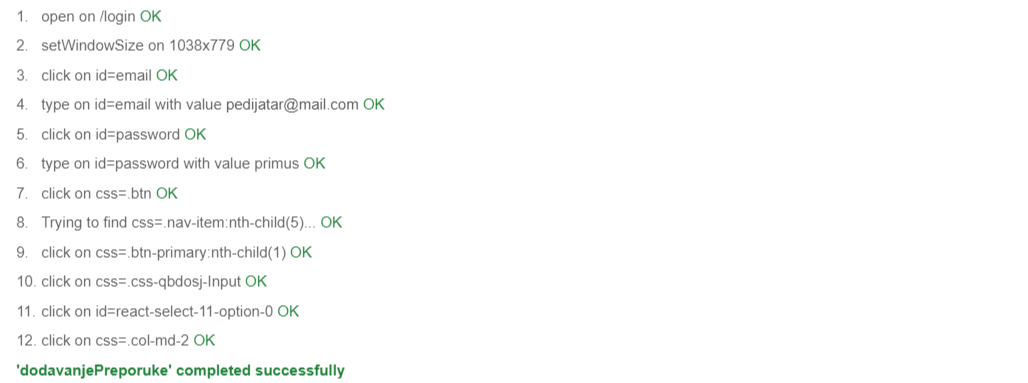
\includegraphics[width=\textwidth]{slike/selenium1.1.png} 
				\caption{Rezultati testiranja grupe koraka 1} 
			\end{figure}

			\begin{figure}[H]
				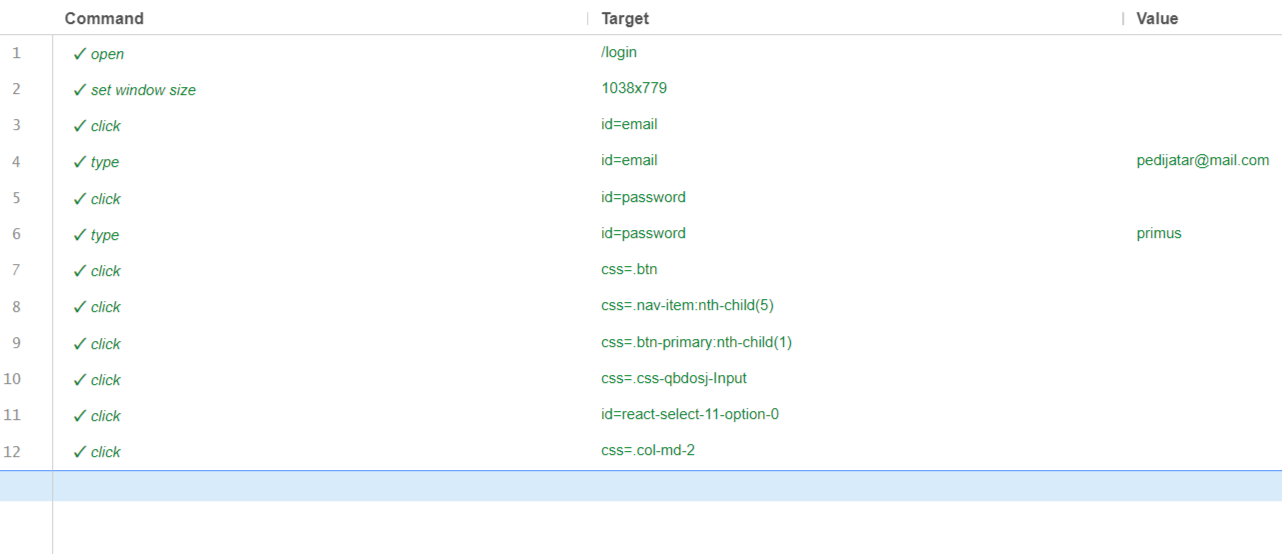
\includegraphics[width=\textwidth]{slike/selenium1.2.png} 
				\caption{Rezultati testiranja grupe koraka 1} 
			\end{figure}

			 \subsubsection*{Grupa koraka 2: Pregled neobrađene preporuke za bolovanje}
			 Koraci:
			 \begin{packed_enum}
				\item Prijava u sustav kao roditelj ("roditelj@mail.com")
				\item Odabir opcije "Bolovanja" iz alatne trake.
				\item Odabir preporuke iz popisa preporuke ("Tamara Stanic 2023-12-25").
			 \end{packed_enum}
			 Očekivani rezultati:
			 \begin{packed_enum}
				\item Roditelj se može prijaviti u sustav.
				\item Postoji opcija "Bolovanja" u alatnoj traci.
				\item Postoji tražena preporuka za bolovanje u popisu preporuka.
				\item Pod "Status" piše "Čeka odobrenje." unutar modalnog ekrana.
			 \end{packed_enum}

			 
			 \begin{figure}[H]
				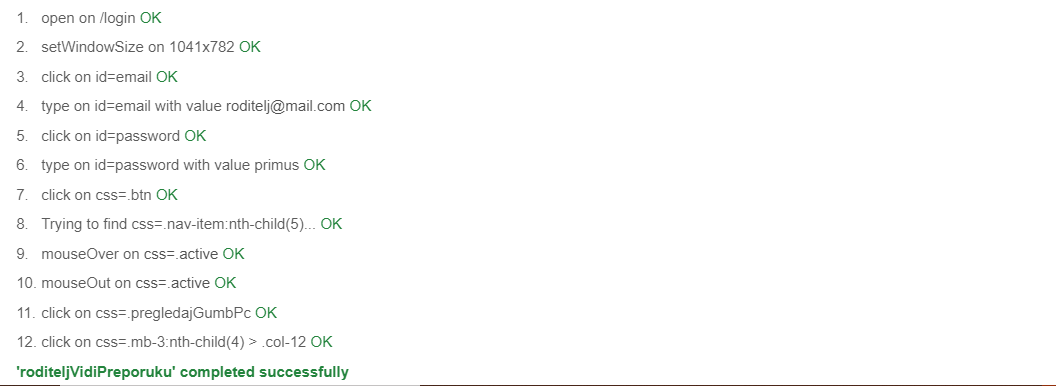
\includegraphics[width=\textwidth]{slike/selenium2.1.png} 
				\caption{Rezultati testiranja grupe koraka 2} 
			\end{figure}

			\begin{figure}[H]
				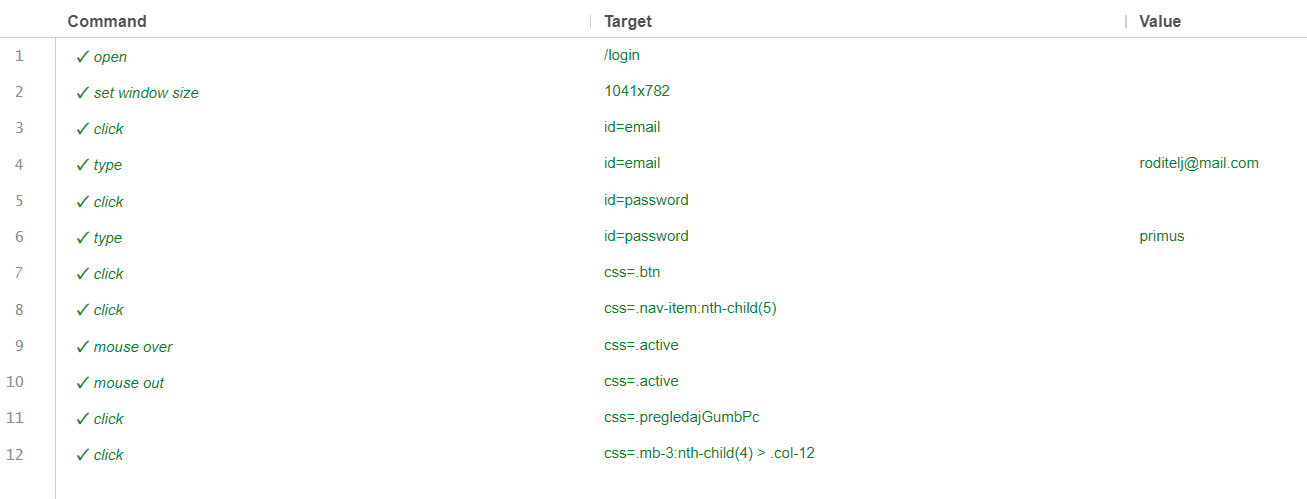
\includegraphics[width=\textwidth]{slike/selenium2.2.png} 
				\caption{Rezultati testiranja grupe koraka 2} 
			\end{figure}

			 \subsubsection*{Grupa koraka 3: Odobravanje preporuke za bolovanje}
			 Koraci:
			 \begin{packed_enum}
				\item Prijava u sustav kao liječnik obiteljske medicine ("doktor@mail.com")
				\item Odabir opcije "Bolovanja" iz alatne trake.
				\item Odabir preporuke iz popisa preporuke ("Tamara Stanic 2023-12-25").
				\item Odabir opcije "Odobri" iz modalnog ekrana.
			 \end{packed_enum}
			 Očekivani rezultati:
			 \begin{packed_enum}
				\item Liječnik obiteljske medicine se može prijaviti u sustav.
				\item Postoji opcija "Bolovanja" u alatnoj traci.
				\item Postoji tražena preporuka za bolovanje u popisu preporuka.
				\item Postoji opcija "Odobri" unutar modalnog okvira.
			 \end{packed_enum}

			 \begin{figure}[H]
				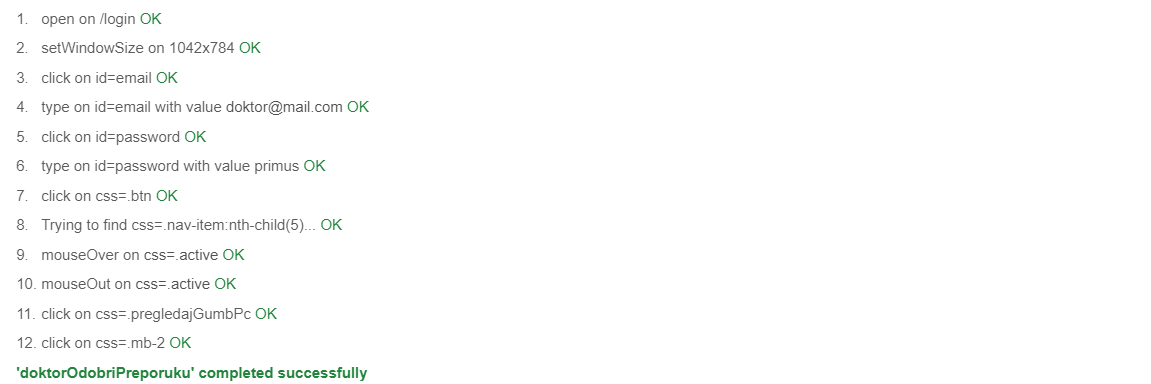
\includegraphics[width=\textwidth]{slike/selenium3.1.png} 
				\caption{Rezultati testiranja grupe koraka 3} 
			\end{figure}

			\begin{figure}[H]
				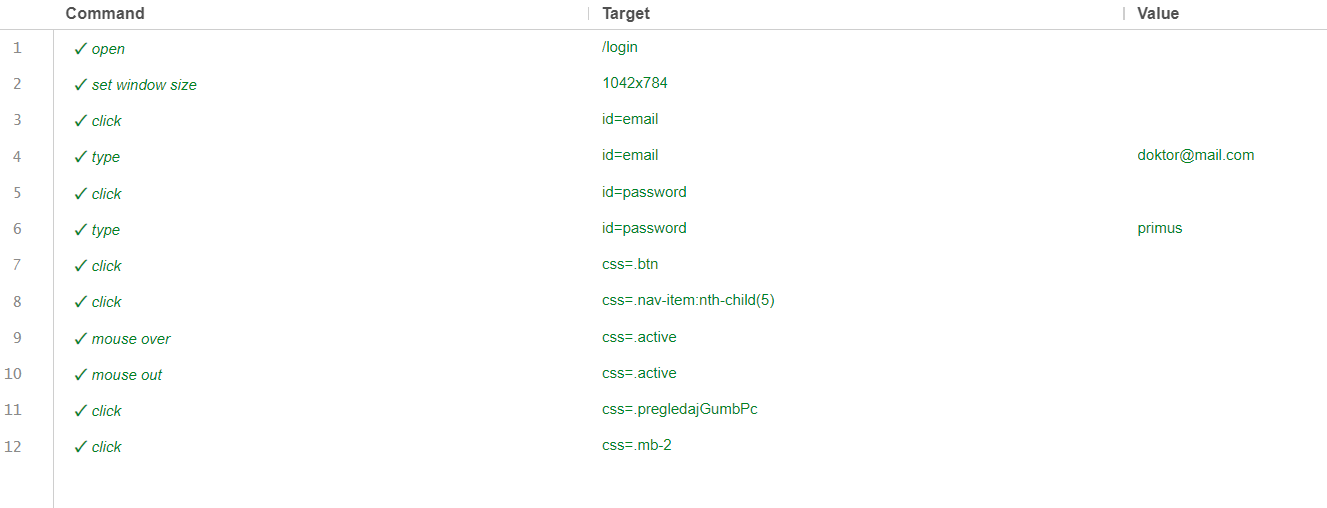
\includegraphics[width=\textwidth]{slike/selenium3.2.png} 
				\caption{Rezultati testiranja grupe koraka 3} 
			\end{figure}

			 \subsubsection*{Grupa koraka 4: Pregled odobrene preporuke za bolovanje}
			 Koraci:
			 \begin{packed_enum}
				\item Prijava u sustav kao roditelj ("roditelj@mail.com")
				\item Odabir opcije "Bolovanja" iz alatne trake.
				\item Odabir preporuke iz popisa preporuke ("Tamara Stanic 2023-12-25").
			 \end{packed_enum}
			 Očekivani rezultati:
			 \begin{packed_enum}
				\item Roditelj se može prijaviti u sustav.
				\item Postoji opcija "Bolovanja" u alatnoj traci.
				\item Postoji tražena preporuka za bolovanje u popisu preporuka.
				\item Pod "Status" piše "Odobreno." u modalnom ekranu preporuke.
			 \end{packed_enum}
			\eject

			\begin{figure}[H]
				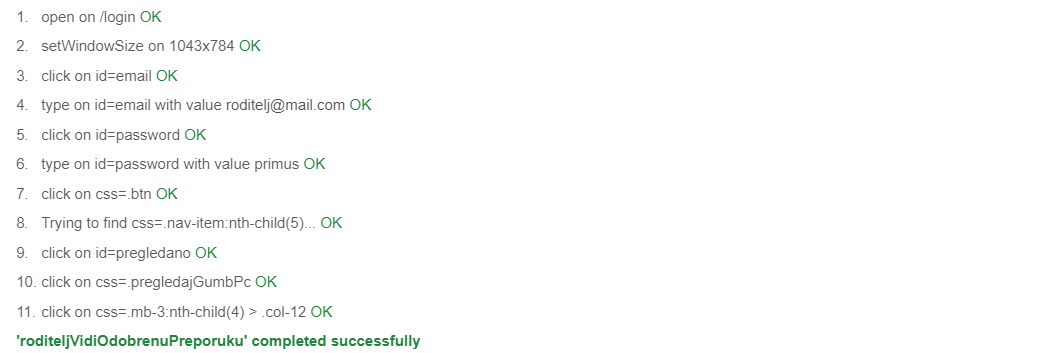
\includegraphics[width=\textwidth]{slike/selenium4.1.png} 
				\caption{Rezultati testiranja grupe koraka 4} 
			\end{figure}

			\begin{figure}[H]
				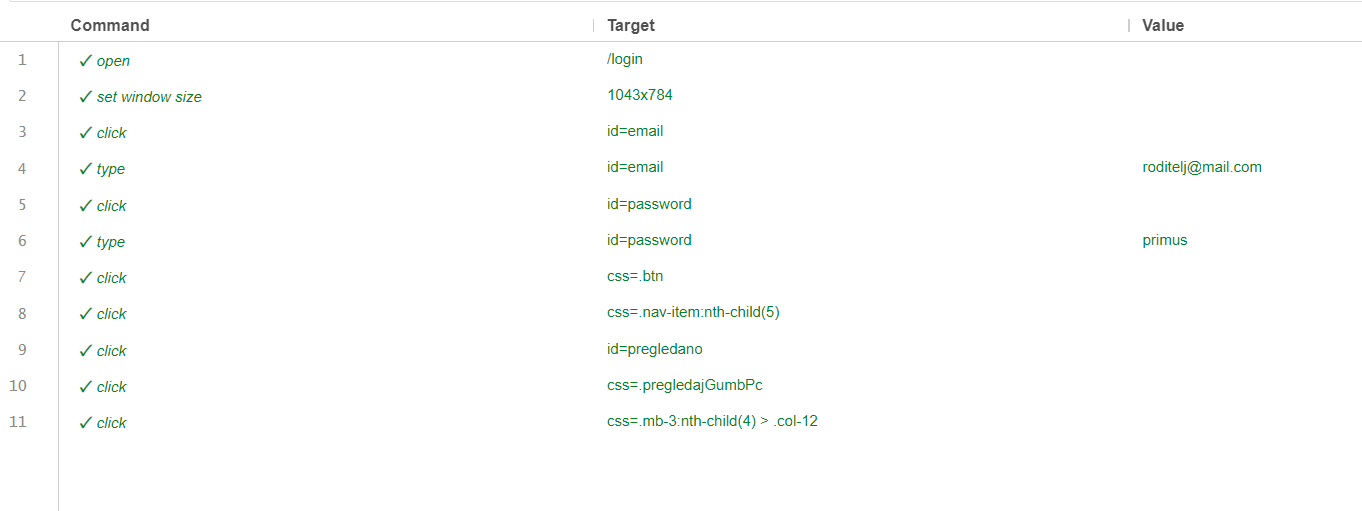
\includegraphics[width=\textwidth]{slike/selenium4.2.png} 
				\caption{Rezultati testiranja grupe koraka 4} 
			\end{figure}
		
		\section{Dijagram razmještaja}
			Dijagrami razmještaja prikazuju konfiguraciju sklopovlja i programske podrške koja se koristi za implementaciju sustava u njegovom operativnom okruženju. Na cloud platformi smješten je poslužitelj baze podataka te web poslužitelji za backend i frontend. Korisnici pristupaju web aplikaciji putem svog web preglednika. Sustav je temeljen na arhitekturi "klijent - poslužitelj" s komunikacijom između korisničkih računala (roditelj, pedijatar, doktor, administrator) i poslužitelja putem HTTPS veze.
			\begin{figure}[H]
				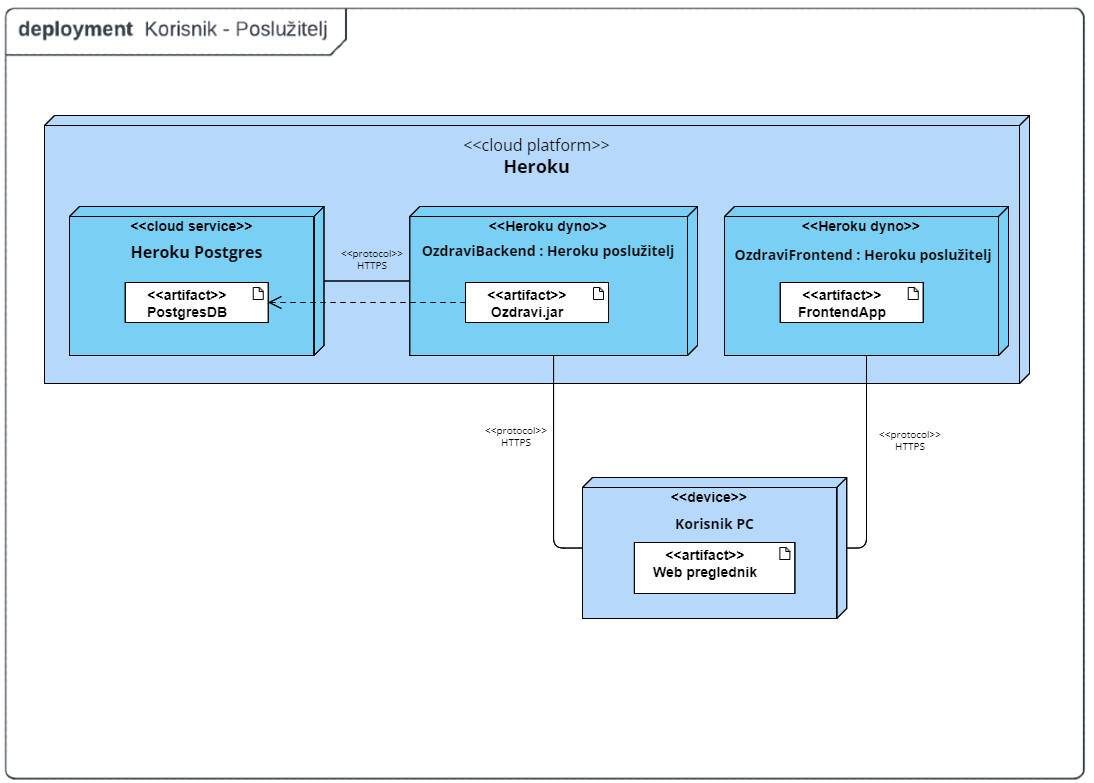
\includegraphics[width=\textwidth]{slike/deploymentDiagram.png} 
				\caption{Dijagram razmještaja} 
			\end{figure}
			\eject 
		
		\section{Upute za puštanje u pogon}
			Aplikacija "Odravi" se sastoji od nekoliko dijelova koje je potrebno postaviti kako bi se pokrenula u lokalnom okruženju.
		
			\subsection*{Postavljanje baze podataka}
			U procesu postavljanja baze podataka za aplikaciju "Ozdravi", prvi korak je instalacija relacijske baze podataka
			\href{https://www.postgresql.org/download/}{\textit{PostgreSQL-a}}. Nakon završetka instalacije, slijedi standardni postupak postavljanja korisničkog imena i lozinke (neobavezno).
			Nakon uspješne instalacije, potrebno je pristupiti konzoli baze (psql) kako bi se stvroili potrebni resursi za rad backenda aplikacije "Ozdravi".
	
			Nakon toga, izvršavaju se sljedeće naredbe:
			\lstinputlisting[style=SQLStyle, caption={Postavljanje baze podataka}]{code/db_setup.sql}

			Sada bi trebala biti stvorena baza podataka "ozdravi", čiji je vlasnik korisnik "welebyte". Naredbom \textit{\textbackslash l} može se provjeriti lista svih postojećih 
			baza podataka i njihovih vlasnika.
			\begin{figure}[H]
				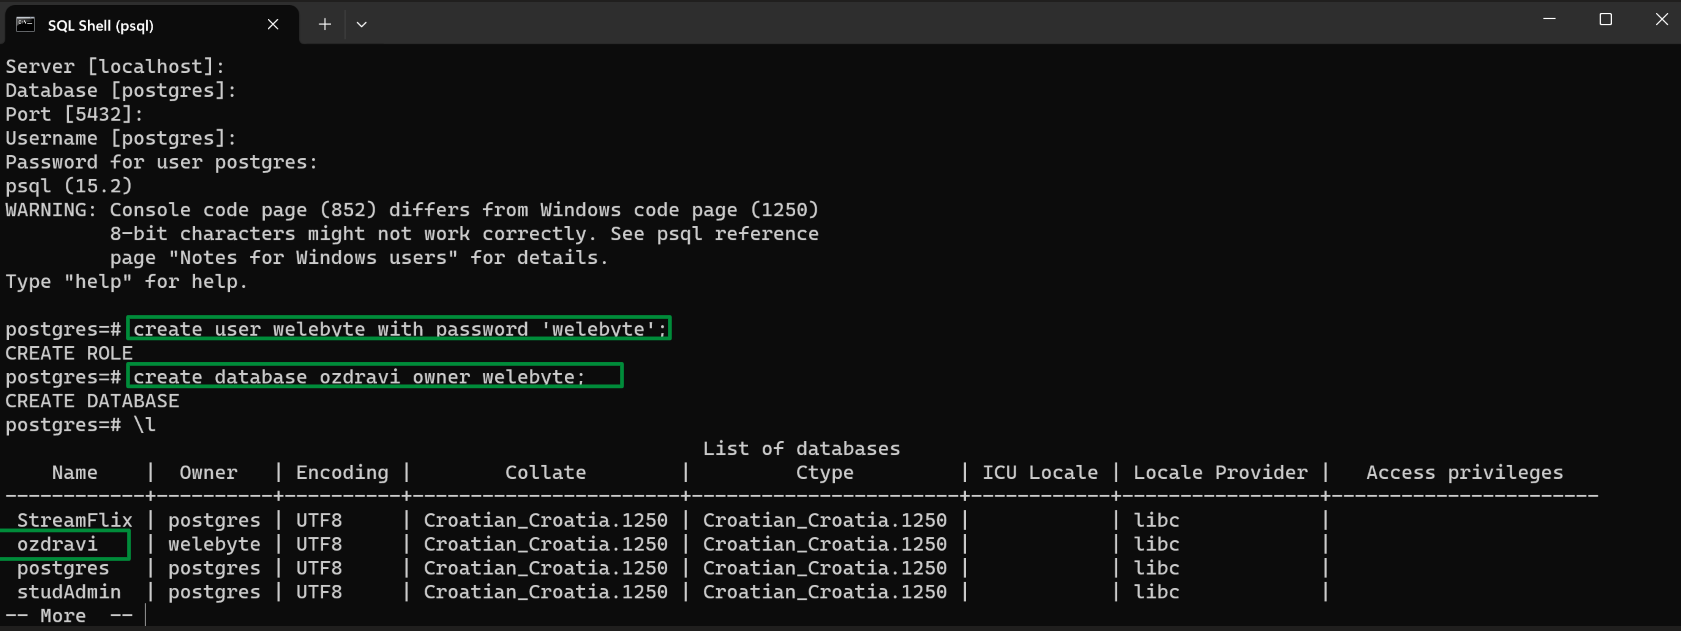
\includegraphics[width=\textwidth]{slike/sqlshell2.png} 
				\caption{Postavljanje baze podataka} 
			\end{figure}
	
			\subsection*{Postavljanje i pokretanje backenda aplikacije}
			Backend aplikacije je pisan u Javi 17, što znači da je na sustavu koji pokreće aplikaciju potrebno imati intaliran JDK (Java Development Kit) - preporučamo \href{https://www.openjdk.org}{\textit{OpenJDK}} kao open-source implementaciju, ali i druge inačica bi trebala raditi.
			Osim Jave, potrebno je imati i \href{https://maven.apache.org/download.cgi}{\textit{Apache Maven}} instaliran. To je alat koji koristimo za upravljenje bibliotekama i "buildovima" backend aplikacije.
			
			Pri pokretanju, potrebno je u konzoli otvoriti mapu \textit{IzvorniKod/ozdravi-backend} a aplikacija se dalje kompajlira izvršavanjem sljedećih naredbi:
			\lstinputlisting[style=ShellStyle, caption={Instalacija i kompajliranje backenda}]{code/mvn_cmd.shell}

			i pokreće pomoću 
			\lstinputlisting[style=ShellStyle, caption={Pokretanje backenda}]{code/java_jar.shell}
			
			Aplikacija je sada dostupna na portu 8080 lokalnog stroja.

			\subsection*{Postavljanje frontenda}
			Frontend aplikacije je pisan u Reactu i za njegovo pakiranje i pokretanje potrebno je preuzeti \href{https://nodejs.org/en/download/}{Node.js}.

			Pri pokretanju, potrebno je u konzoli otvoriti mapu \textit{IzvorniKod/ozdravi-frontend} i izvršiti sljedeće naredbe:
			\lstinputlisting[style=ShellStyle, caption={Instalacija i pokretanje frontenda}]{code/npm_cmd.shell}

			Prvu je naredbu potrebno izvršiti samo jednom, kako bi se prikupili potrebni paketi, a druga je naredba ona koja pokreće server na kojem je frontend dostupan za preuzimanje.
			
			\newpage \noindent Nakon pokretanja, aplikaciju je moguće vidjeti na adresi: \url{http://localhost:3000.}\\
			\begin{figure}[H]
				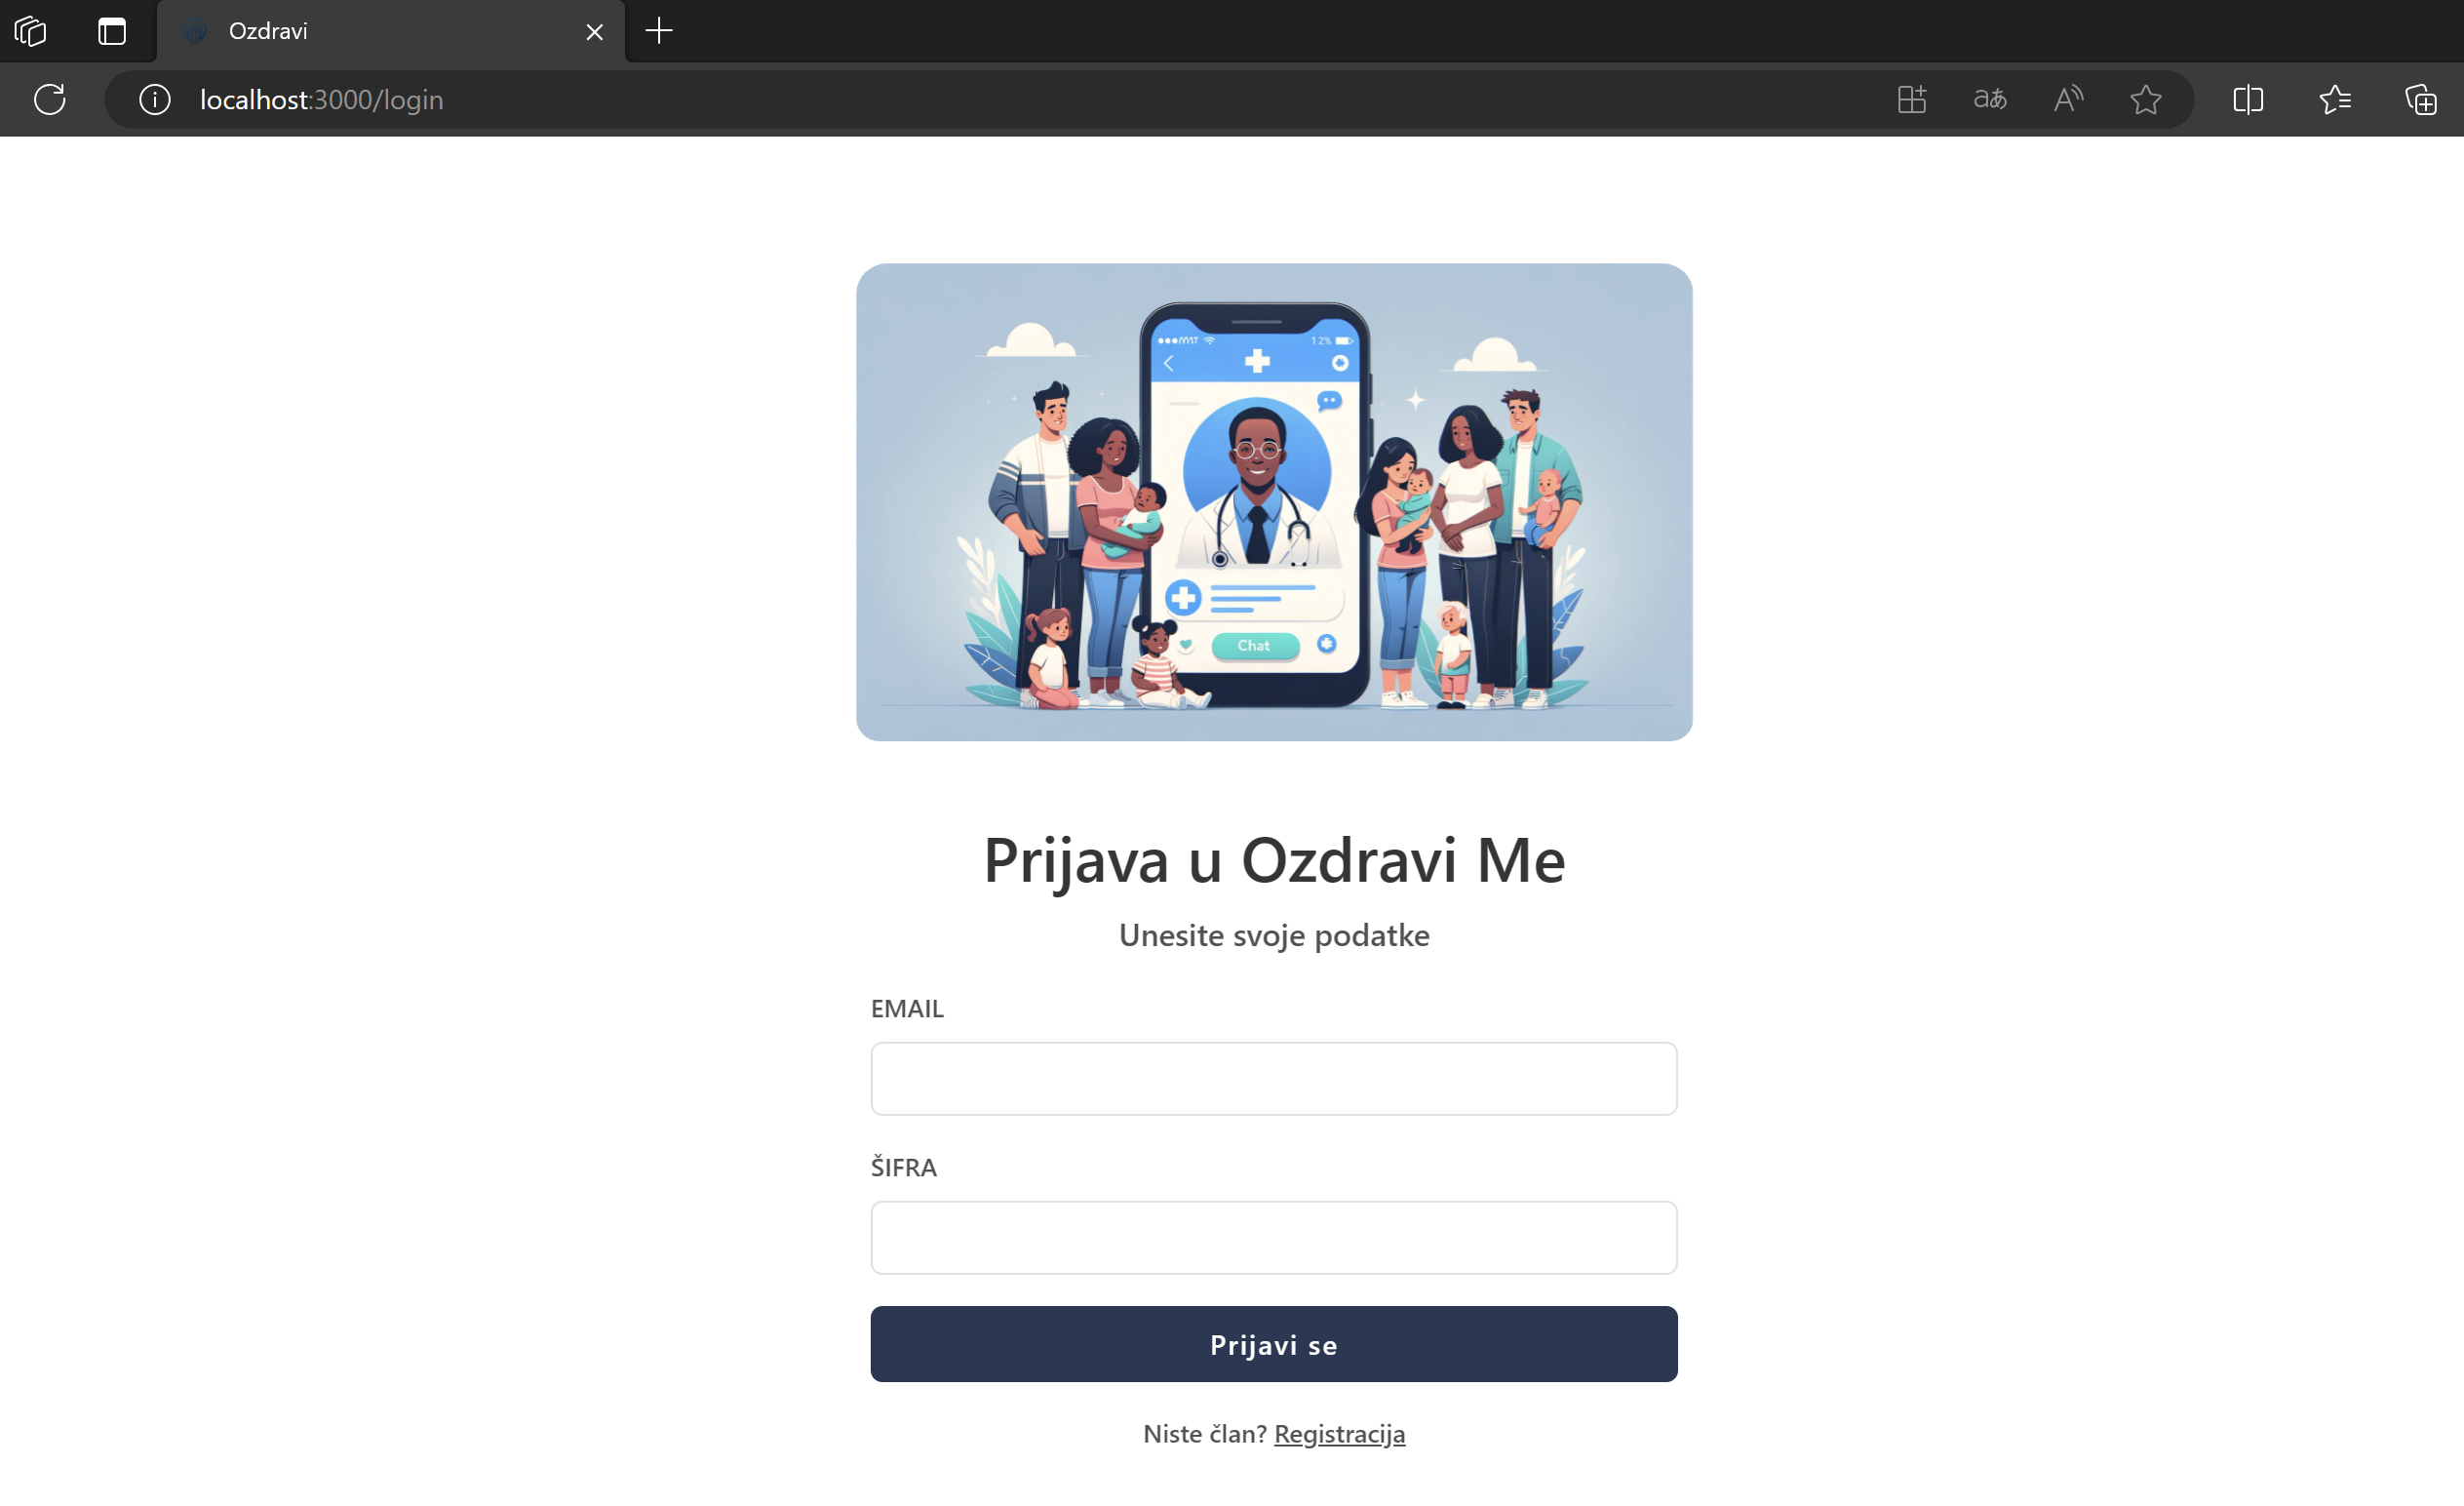
\includegraphics[width=\textwidth]{slike/loc3000.png} 
				\caption{Aplikacija na portu 3000} 
			\end{figure}
			Nakon svake promjene i spremanja koda, stranica se automatski ponovno učitava. Osim toga, postoji mogućnost promjene porta aplikacije uređivanjem datoteke \textit{package.json}, 
			gdje se u liniji koda \textit{"start": set PORT=3006 \&\& react-scripts start} može izmijeniti broj porta prema želji.
			
			
			\subsubsection*{Stvaranje PDF izvještaja dokumentacije}
			Dokumentacija za ovaj projekt je napisana pomoću paketa \LaTeX  i nalazi se u mapi \textit{Dokumentacija/}. Kako bi se iz .tex datoteka izgradio PDF izvješaj potrebno je na računalu imati instalaciju \LaTeX-a i pokrenuti ispravne naredbe za izgradnju PDF-a (npr \textit{latexmk}).
			\eject 
	\chapter{Zaključak i budući rad}
		
		%dio 2. revizije
		
		 %U ovom poglavlju potrebno je napisati osvrt na vrijeme izrade projektnog zadatka, koji su tehnički izazovi prepoznati, jesu li riješeni ili kako bi mogli biti riješeni, koja su znanja stečena pri izradi projekta, koja bi znanja bila posebno potrebna za brže i kvalitetnije ostvarenje projekta i koje bi bile perspektive za nastavak rada u projektnoj grupi.
		
		 %Potrebno je točno popisati funkcionalnosti koje nisu implementirane u ostvarenoj aplikaciji.

		 Zadatak grupe bio je razvoj web-aplikacije Ozdravi. Projekt "Ozdravi" predstavlja značajan korak prema modernizaciji zdravstvenog sustava, omogućujući brži pristup informacijama, efikasnije upravljanje resursima te bolje praćenje zdravstvenih podataka. Tijekom 13 tjedana rada, tim je uspješno implementirao zadanu web aplikaciju. Provedba projekta bila je podijeljena u tri faze. \\
		 Prva faza, poznata kao faza inicijacije \textit{(en. initiation)}, predstavlja početak cijelog procesa razvoja. Provedeno je formiranje tima, nakon čega je uslijedilo detaljno upoznavanje sa zadatkom. Time su članovi tima stekli jasnu sliku o svrsi aplikacije, funkcionalnostima i korisničkim zahtjevima. U ovoj fazi odabrane su odgovarajuće tehnologije i alati.   
		 Druga faza projekta, odnosno faza otkrivanja \textit{(engl. discovery)}, obilježena je strukturiranim pristupom definiranja zahtjeva i dokumentacijom, što je značajno olakšalo implementaciju u drugoj fazi. Prvi samostalni zadaci članova tima uključivali su usvajanje znanja o odabranim tehnologijama i alatima. Izrada vizualnih prikaza idejnih rješenja problemskog zadatka pomogla je u rješavanju nedoumica oko implementacije rješenja. Obrasci uporabe, sekvencijski dijagrami te modeli baze podataka bili su ključni u usmjeravanju podtimova zaduženih za razvoj backenda i frontenda. \\
		 U trećoj fazi, poznata kao faza isporuke \textit{(engl. delivery)}, naglasak je bio na samostalnom radu članova tima na implementaciji i dokumentaciji. Kvalitetna dokumentacija olakšat će buduće prilagodbe sustava te omogućiti korisnicima lakše korištenje aplikacije. Osim realizacije rješenja, u ovoj fazi bilo je potrebno izraditi ostale UML dijagrame te popratnu dokumentaciju kako bi se budućim korisnicima omogućilo jednostavnije korištenje te izvršenje potrebnih preinaka sustava. 
		 Redoviti sastanci tima pridonijeli su informiranosti o napretku projekta, izvrsnoj organizaciji te učinkovitoj podjeli zadataka. \\
		 Nakon uspješne implementacije, projekt "Ozdravi" otvara prostor za daljnje poboljšanje i proširenje. U skladu s time, moguće je izvesti refaktorizaciju određenih dijelova koda kako bi se smanjio tehnički dug i poboljšala održivost aplikacije. Također, razmatra se unapređenje deployment okruženja kako bi se postigle bolje performanse i povećala dostupnost sustava.
		 Potencijalno proširenje funkcionalnosti sustava obuhvaća implementaciju mobilne aplikacije, pružajući dodatnu fleksibilnost korisnicima. Nadogradnja dodatnim funkcionalnostima ključna je u zadovoljavanju potreba korisnika, omogućavajući dodavanje novih značajki koje će obogatiti korisničko iskustvo. Uz to, postoji mogućnost unapređenja korisničkog sučelja (UI) i korisničkog iskustva (UX), čime će se poboljšati funkcionalnost sustava. S kontinuiranim praćenjem povratnih informacija korisnika, osigurat će se da aplikacija "Ozdravi" uvijek bude u skladu s najvišim standardima i potrebama moderne zdravstvene tehnologije. \\
		 Sudjelovanje u projektu "Ozdravi" pružilo je vrijedno iskustvo članovima tima, naglašavajući važnost suradnje, organizacije te kontinuiranog učenja u radu na složenim projektima.
		\eject 
	\chapter*{Popis literature}
		\addcontentsline{toc}{chapter}{Popis literature}
	 	
 		%Kontinuirano osvježavanje
	
		%Popisati sve reference i literaturu koja je pomogla pri ostvarivanju projekta.
		
		
		\begin{enumerate}
			
			
			\item  Programsko inženjerstvo, FER ZEMRIS, \url{http://www.fer.hr/predmet/proinz}
			
			\item  I. Sommerville, "Software engineering", 8th ed, Addison Wesley, 2007.
			
			%\item  T.C.Lethbridge, R.Langaniere, "Object-Oriented Software Engineering", 2nd ed. McGraw-Hill, 2005.
			
			%\item  I. Marsic, Software engineering book``, Department of Electrical and Computer Engineering, Rutgers University, \url{http://www.ece.rutgers.edu/~marsic/books/SE}
			
			%\item  The Unified Modeling Language, \url{https://www.uml-diagrams.org/}
			
			%\item  Astah Community, \url{http://astah.net/editions/uml-new}
		\end{enumerate}
		
		 
	
	\begingroup
	\renewcommand*\listfigurename{Indeks slika i dijagrama}
	%\renewcommand*\listtablename{Indeks tablica}
	%\let\clearpage\relax
	\listoffigures
	%\vspace{10mm}
	%\listoftables
	\endgroup
	\addcontentsline{toc}{chapter}{Indeks slika i dijagrama}

	\eject 
	\chapter*{Dodatak: Prikaz aktivnosti grupe}
		\addcontentsline{toc}{chapter}{Dodatak: Prikaz aktivnosti grupe}
		
		\section*{Dnevnik sastajanja}
		
		\begin{packed_enum}
			\item  sastanak
			
			\item[] \begin{packed_item}
				\item Datum: \date[{19. listopada 2023.} %%zas ovdje ide ova sintaksa [
				\item Prisustvovali: D. Matić, L. Crvelin, V. Kumanović, M. Lešković, K. Valečić, M. Vidaković
				\item Trajanje: 35min
				\item Teme sastanka:
				\begin{packed_item}
					\item  izbor tehnologije
					\item  izbor teme
                    \item  ime tima
                    \item  osnovna podjela posla
                    \item  osiguravanje pristupa na sve servisa svim članovima tima
				\end{packed_item}
            \item Zaključak: \\Dogovoreni su taskovi za prvi sprint (do četvrtrka 26.10). Oni za većinu ljudi uključuju učenje gita i tehnologija koje su odabrali (backend/frontend), a L. Crvelin treba i napraviti prve korake u organizaciji dokumentacije. Voditelj D. Matić će postaviti repozitorij na GitHubu i osigurati svima pristup. Dogovorena je i radionica na temu značajki (featurea) aplikacije sutra u 12 sati, gdje ćemo pokušati prioritizirati posao i složiti Jiru.
			\end{packed_item}

   
			\item  sastanak
			\item[] \begin{packed_item}
				\item Datum: \date[{20. listopada 2023.}
				\item Prisustvovali:  D. Matić, L. Crvelin, V. Kumanović, M. Lešković, K. Valečić, M. Vidaković
				\item Trajanje: 1h 45min
				\item Teme sastanka:
				\begin{packed_item}
					\item  analiziranje značajki aplikacije i napisati iz njih epice i storije u Jiri
					\item  stvaranje dijagrama
                    \item  daljnja podjela posla
				\end{packed_item}
            \item Zaključak: \\Detaljno su analizirane značajke aplikacije i stvoreni dijagrami iz kojih se može stvoriti definicija baze podataka što će do kraja sprinta učiniti V. Kumanović i prioritizirani popis zadataka koji će u Jiri stvoriti D. Matić. Također, identificirali smo nejasnoće u samoj definiciji zadatka koje ćemo prenijeti asistentici.
            M. Vidaković će do kraja sprinta istražiti kako se pravilno postavlja Spring projekt, a K. Valečić će isto učiniti za React u čemu će mu pomoći M. Lešković. \\
            Dogovorene su još dvije radionice sljedeći tjedan, u četvrtak i petak na temu postavljanja Reacta i Springa.
			\end{packed_item}


            \item  sastanak
			\item[] \begin{packed_item}
				\item Datum: \date[{26. listopada 2023.}
				\item Prisustvovali: D. Matić, L. Crvelin, L. Cvetkovski, V. Kumanović, M. Lešković, K. Valečić, M. Vidaković 
				\item Trajanje: 1h 30min
				\item Teme sastanka:
				\begin{packed_item}
					\item  planiranje i praćenje napretka
					\item  postavljanje backend-a prema svim pravilima i omogućavanje nesmetanog razvoja u budućnosti.
				\end{packed_item}
            \item Zaključak: \\
            Potvrdili smo da svi imaju potreban pristup na JIRU i GitHub repozitoriju. \\
             L. Crvelin je izložila napredak u dokumentiranju i predstavila način prikupljanja podataka za pojedine dijelove dokumentacije. Podaci o napretku će se prikupljati kroz komentare na JIRA taskovima i kroz bilješke sa sastanaka. Sljedeći koraci vezani uz izradu dokumentacije su raspisivanje obrazaca uporabe i pisanje opisa projektnog zadatka. To će preuzeti L. Crvelin i V. Kumanović. Također, L. Crvelin je naglasila važnost praćenja potrošenog vremena za svaki zadatak koji radimo. To će u JIRI postaviti D. Matić. \\
             Predstavljena je i schema baze podataka koju smo komentirali i utvrdili koje su potrebne promjene. Te će promjene u ovom sprintu učiniti V. Kumanović i M. Vidaković te će ih predstaviti timu na sljedećem planiranju sprinta u četvrtak. \\
             M. Vidaković je prezentirala napredak vezan uz postavljanje Spring backenda i preuzela zadatak integracije backenda s Postgresom što se može događati usporedno uz razvijanje scheme baze. \\
             K. Valečić i M. Lešković su potvrdili da su spremni za nadolazeću radionicu vezanu uz postavljanje Reacta, koja će se održati sutra (petak, 27.10. u 14 sati). Nakon te radionice bit ćemo spremni za početak razvoja na frontendu, što će preuzeti L. Cvetkovski i K. Valečić. \\
             Komentirali smo rad s gitom te je M. Lešković pokazao workflow u GitHub Desktop alatu. Naglašena je važnost da više ljudi pogleda PR prije mergea s glavnom granom.
            
			\end{packed_item}

               \item  sastanak
			\item[] \begin{packed_item}
				\item Datum: \date[{27. listopada 2023.}
				\item Prisustvovali:  D. Matić, L. Crvelin, L. Cvetkovski, V. Kumanović, M. Lešković, K. Valečić
				\item Trajanje: 45min
				\item Teme sastanka:
				\begin{packed_item}
					\item  planiranje i praćenje napretka
					\item  postavljanje frontend-a prema svim pravilima i omogućavanje nesmetanog razvoja u budućnosti
				\end{packed_item}
            \item Zaključak: \\
            M. Lešković je postavio temelje React projekta i detaljno objasnio što i kako radi. Dogovorili smo se da ćemo za izgradnju korisničkog sučelja koristiti Bootstrap, a integraciju Bootstrapa s projektom će napraviti L. Cvetkovski. Za to vrijeme će K. Valečić naučiti kako se Bootstrap koristi i onda s L. Cvetkovski izgraditi prvih nekoliko stranica aplikacije (login/register, homepage, profile edit page) do kraja ovog sprinta. M. Lešković će od sad raditi na backend dijelu. \\
            Dogovorili smo se da ćemo dodati README na projekt s uputama kako pokrenuti backend / frontend. To je bitno da svi mogu jednostavno postaviti projekt na svojim računalima.
			\end{packed_item}

            \item  sastanak
			\item[] \begin{packed_item}
				\item Datum: \date[{31. listopada 2023.}
				\item Prisustvovali:  D. Matić, L. Crvelin, L. Cvetkovski, V. Kumanović, M. Lešković, K. Valečić, M. Vidaković
				\item Trajanje: 45min
				\item Teme sastanka:
				\begin{packed_item}
					\item  praćenje napretka na frontendu
					\item  pregled funkcionalnih zahtjeva
				\end{packed_item}
                \item Zaključak: \\
                L. Crvelin je pokazala dosadašnji napredak vezan uz definiranje funkcionalnih zahtjeva i izložila nejasnoće koje imamo u ovom trenutku. Kroz raspravu smo razjasnili sve i omogućili daljnji razvoj dokumentacije.
                L. Cvetkovski je pokazao napredak vezan uz razvoj frontenda. Dogovoreno je da će frontend tim imati zasebne sastanke u terminu u kojem se dogovore kako bi odredili sljedeće korake.
            
			\end{packed_item}

            \item  sastanak
			\item[] \begin{packed_item}
				\item Datum: \date[{1. studenoga 2023.}
				\item Prisustvovali: L. Crvelin, L. Cvetkovski, M. Lešković
				\item Trajanje: 1h
				\item Teme sastanka:
				\begin{packed_item}
					\item  Razdvajanje uloga
                    \item Određivanje podstranica za svaku ulogu
                    \item Pregled dosadašnjeg napretka
                    \item podjela zadatka
				\end{packed_item}
                \item Zaključak: \\
                Dogovoreno je da trebamo razdvojiti uloge na platformi, odnosno definirati različite korisničke uloge: pedijatar, liječnik obiteljske medicine (OM), i roditelj.
                Razgovarali smo o potrebi definiranja specifičnih podstranica za svaku ulogu kako bismo omogućili prilagođeni sadržaj i funkcionalnosti za svaku kategoriju korisnika.
                Odlučeno je da će adminu biti omogućeno upravljanje svim računima korisnika s jedne centralne stranice nazvane "racuni.js". Ovo će pojednostaviti administraciju i omogućiti efikasnije upravljanje korisničkim računima.
                Razgovarali smo o raspodjeli zadatka za izradu osnovnih kostura stranica za svaku ulogu na frontendu. L. Cvetkovski će raditi na stranici za pedijatra i liječnika obiteljske medicine, a K. Valečić će raditi na stranici za roditelja.
			\end{packed_item}

            \item  sastanak
			\item[] \begin{packed_item}
				\item Datum: \date[{1. studenoga 2023.}
				\item Prisustvovali: D. Matić, M. Vidaković
				\item Trajanje: 45min
				\item Teme sastanka: 
				\begin{packed_item}
					\item  projektiranje baze podataka
				\end{packed_item}
                \item Zaključak: \\
                
			\end{packed_item}
			

            \item  sastanak
			\item[] \begin{packed_item}
				\item Datum: \date[{2. studenoga 2023.}
				\item Prisustvovali: D. Matić, L. Crvelin, L. Cvetkovski, V. Kumanović, M. Lešković, K. Valečić, M. Vidaković
				\item Trajanje: 2h 45min
				\item Teme sastanka: 
				\begin{packed_item}
					\item  planiranje i praćenje napretka
				\end{packed_item}
                \item Zaključak: \\
                Dogovorili smo sljedeće korake koje treba napraviti vezano uz dokumentaciju kako bismo mogli tražiti povratnu
                informaciju na konzulatcijama u utorak (7.11). L. Crvelin će prepisati definirane tablice baze iz Excela u
                dokumentaciju, a V. Kumanović će iz definiranih tablica nacrtati dijagram baze podataka koji je također dio
                dokumentacije. Prošli smo kroz sve obrasce uporabe koje smo do sad definirali i dogovorili se da će oni biti dovršeni do
                ponedjeljka, što će učiniti L. Crvelin. \\
                
                D. Matić je pokazao napredak u izboru i postavljanju deploy platforme. Izabrali smo Heroku i napravili osnovno
                postavljenje dviju aplikacija (frontend i backend). \\
                
                M. Vidaković je pokazala kako se Postgres baza spaja na Spring aplikaciju što nam je bio preduvjet da možemo nastaviti
                razvoj na backendu, ali i da možemo napraviti potpun deployment aplikacije. Nastavno na to će M. Lešković
                implementirati mehanizme za prijavu i registraciju korisnika pomoću Spring Security modula, a D. Matić će napraviti
                potrebne korake na Heroku platformi vezane uz deploy aplikacije. M. Vidaković će u sljedećem sprintu implementirati
                mehanizam uloga na entitetu korisnika. \\
                
                L. Cvetkovski i K. Valečić su podijelili plan za razvoj frontenda s ostalima. Potvrdili smo daljnje korake
                vezane uz razvoj React aplikacije koji uključuju restrukturiranje i razvoj homescreena. Dogovoreno je da će frontend tim
                razraditi najbolje načine kako nastaviti raditi s obzirom da backend još uvijek zaostaje za frontendom.
               
			\end{packed_item}

			\item  sastanak
			\item[] \begin{packed_item}
				\item Datum: \date[{9. studenoga 2023.}
				\item Prisustvovali: D. Matić, L. Crvelin, L. Cvetkovski, V. Kumanović, M. Lešković, K. Valečić, M. Vidaković
				\item Trajanje: 1h 30min
				\item Teme sastanka: 
				\begin{packed_item}
					\item  planiranje i praćenje napretka
				\end{packed_item}
                \item Zaključak: \\
				Analizirali smo povratne informacije koje smo dobili na konzultacijama u utorak i podijelili posao vezan uz to 
				u ovom sprintu. L. Crvelin će napraviti sve potrebne promjene na UC-ovima,  Vedran Kumanović će modificirati dijagram 
				baze podataka, a Dorian Matić će dovršiti odlomak "Arhitektura sustava". \\
 
				Leon Cvetkovski je predstavio napredak u refaktoriziranju frontenda koji su on i Krešimir Valečić napravili u ovom sprintu.
				Zaključili smo da je frontend sad spreman za spajanje s backendom. \\
				 
				Mihael Lešković je opisao probleme s kojima se susreo pri postavljanju Spring Security modula za backend aplikacije. 
				Dogovoreno je da će on i Dorian Matić probati što prije to popraviti i omogućiti daljnju razvoj frontenda.
               
			\end{packed_item}

			\item  sastanak
			\item[] \begin{packed_item}
				\item Datum: \date[{11. studenoga 2023.}
				\item Prisustvovali: D. Matić, L. Cvetkovski, M. Lešković, K. Valečić
				\item Trajanje: 1h 30min
				\item Teme sastanka: 
				\begin{packed_item}
					\item  Omogućiti frontend timu da spoji React aplikaciju s backendom
				\end{packed_item}
                \item Zaključak: \\
                Predstavljen je dio backenda vezan uz Spring Security. Frontend tim je naučio kako se pokreće backend aplikacija lokalno.
                Dogovoreni su sljedeći koraci.
				
               
			\end{packed_item}

			\item  sastanak
			\item[] \begin{packed_item}
				\item Datum: \date[{16. studenoga 2023.}
				\item Prisustvovali: D. Matić, L. Crvelin, L. Cvetkovski, V. Kumanović, M. Lešković, K. Valečić, M. Vidaković
				\item Trajanje: 45min
				\item Teme sastanka: 
				\begin{packed_item}
					\item  planiranje i praćenje napretka
				\end{packed_item}
                \item Zaključak: \\
                Timovi za dokumentaciju, backend i frontend su predstavili svoj napredak u ovom sprintu. Dogovorene su zadnje promjene
				u dokumentaciji prije verzije 1.0.\\
				Dogovoreno je da sljedeći sprint zbog međuispita kreće tek u četvrtak, 30.11. Do tad, svi timovi trebaju smisliti
				prijedloge daljenjeg djelovanja. Svi članovi tima su pristali na cilj da cjelokupna funkcionalnost aplikacije bude
				gotova do 1.1.2024.
                
               
			\end{packed_item}

			\item  sastanak
			\item[] \begin{packed_item}
				\item Datum: \date[{30. studenoga 2023.}
				\item Prisustvovali: D. Matić, L. Cvetkovski, V. Kumanović, M. Lešković, K. Valečić, M. Vidaković
				\item Trajanje: 40min
				\item Teme sastanka: 
				\begin{packed_item}
					\item  planiranje i praćenje napretka
				\end{packed_item}
                \item Zaključak: \\
                Dogovoreni su daljni koraci za frontend, backend i dokumentaciju. Vedran Kumanović će istražiti koji su nam 
				dijagrami potrebni u dokumentaciji i koji podaci nam trebaju kako bismo ih izradili. Analizirat će kako te 
				podatke prikupiti i imamo li ih već prikupljene. Osim toga, napisat će i odlomak "Upute za puštanje u rad aplikacije"
				 u dokumentaciji, na temelju README-ja. \\
 				Mihael Lešković će nastaviti razvijati podršku za usere tako što će implementirati sve atribute usera unutar 
				aplikacije i također njihove validacije. Mia Vidaković će nastaviti raditi na implementaciji uloga unutar aplikacije.\\
 				Krešimir Valečić i Leon Cvetkovski će nadograditi ekran za registraciju s novim poljima koja su potrebna i napravit 
				će novi ekran za unos ili izmjenu atributa usera.
			
			\end{packed_item}

			\item  sastanak
			\item[] \begin{packed_item}
				\item Datum: \date[{4. prosinca 2023.}
				\item Prisustvovali: D. Matić, M. Lešković, K. Valečić, M. Vidaković
				\item Trajanje: 40min
				\item Teme sastanka: 
				\begin{packed_item}
					\item  
				\end{packed_item}
                \item Zaključak: \\
                
			
			\end{packed_item}

			\item  sastanak
			\item[] \begin{packed_item}
				\item Datum: \date[{7. prosinca 2023.}
				\item Prisustvovali: D. Matić, L. Crvelin, V. Kumanović, M. Lešković, K. Valečić, M. Vidaković
				\item Trajanje: 1h 5min
				\item Teme sastanka: 
				\begin{packed_item}
					\item  planiranje i praćenje napretka
				\end{packed_item}
                \item Zaključak: \\
                Dogovoreno je da će se tijekom sljedećeg sprinta napraviti radionica vezana uz preostale dijagrame koje treba nacrtati
tim za dokumentaciju će predstaviti kakvi su to dijagrami i prikupiti informacije potrebne da ih se nacrta.\\

Vedran Kumanović mora završtiti odlomak "Upute za puštanje u rad aplikacije", što mu je ostalo od prethodnog sprinta.\\

Leon Cvetkovski i Krešimir Valečić moraju završiti ekrane koji su im ostali od prošlog sprinta i nastaviti raditi na
ekranima za preglede i spajanje doktora i pacijenata.\\

Mia Vidaković će nastaviti s implementacijama uloga, a Mihael Lešković će nastaviti rad na korisnicima i pregledima.
                
			
			\end{packed_item}

			\item  sastanak
			\item[] \begin{packed_item}
				\item Datum: \date[{11. prosinca 2023.}
				\item Prisustvovali: 
				\item Trajanje: 
				\item Teme sastanka: 
				\begin{packed_item}
					\item  mid-sprint sync
				\end{packed_item}
                \item Zaključak: \\
                
			
			\end{packed_item}

			\item  sastanak
			\item[] \begin{packed_item}
				\item Datum: \date[{14. prosinca 2023.}
				\item Prisustvovali: 
				\item Trajanje:
				\item Teme sastanka: 
				\begin{packed_item}
					\item  planiranje i praćenje napretka
				\end{packed_item}
                \item Zaključak: \\
                
			
			\end{packed_item}

			\item  sastanak
			\item[] \begin{packed_item}
				\item Datum: \date[{18. prosinca 2023.}
				\item Prisustvovali: D. Matić, L. Crvelin, V. Kumanović, K. Valečić, M. Vidaković
				\item Trajanje: 30min
				\item Teme sastanka: 
				\begin{packed_item}
					\item  mid-sprint sync
				\end{packed_item}
                \item Zaključak: \\
                
			
			\end{packed_item}
		\end{packed_enum}
		
		\eject
		\section*{Tablica aktivnosti}
			 %Doprinose u aktivnostima treba navesti u satima po članovima grupe po aktivnosti.}

			\begin{longtblr}[
					label=none,
				]{
					vlines,hlines,
					width = \textwidth,
					colspec={X[7, l]X[1, c]X[1, c]X[1, c]X[1, c]X[1, c]X[1, c]X[1, c]}, 
					vline{1} = {1}{text=\clap{}},
					hline{1} = {1}{text=\clap{}},
					rowhead = 1,
				} 
			
				\SetCell[c=1]{c}{} & \SetCell[c=1]{c}{\rotatebox{90}{\textbf{Dorian Matić}}} & \SetCell[c=1]{c}{\rotatebox{90}{\textbf{Lucia Crvelin }}} &	\SetCell[c=1]{c}{\rotatebox{90}{\textbf{Leon Cvetkovski }}} & \SetCell[c=1]{c}{\rotatebox{90}{\textbf{Vedran Kumanović }}} &	\SetCell[c=1]{c}{\rotatebox{90}{\textbf{Mihael Lešković }}} & \SetCell[c=1]{c}{\rotatebox{90}{\textbf{Krešimir Valečić }}} &	\SetCell[c=1]{c}{\rotatebox{90}{\textbf{Mia Vidaković }}} \\  
				Upravljanje projektom 		& 4.5 &  &  &  &  &  & \\ 
				Opis projektnog zadatka 	&  & 3.5 &  &  &  &  & \\ 
				
				Funkcionalni zahtjevi       &  & 3 &  &  &  &  &  \\ 
				Opis pojedinih obrazaca 	&  & 8 &  &  &  &  &  \\ 
				Dijagram obrazaca 			&  & 5 &  &  &  &  &  \\ 
				Sekvencijski dijagrami 		&  & 4.5 &  &  &  &  &  \\ 
				Opis ostalih zahtjeva 		&  & 1 &  &  &  &  &  \\ 

				Arhitektura i dizajn sustava	 & 3 &  &  &  &  &  &  \\ 
				Baza podataka				& 2 &  &  & 5 &  &  & 3  \\ 
				Dijagram razreda 			&  &  &  & 2.5 &  &  & 1  \\ 
				Dijagram stanja				&  &  &  &  &  &  &  \\ 
				Dijagram aktivnosti 		&  &  &  &  &  &  &  \\ 
				Dijagram komponenti			&  &  &  &  &  &  &  \\ 
				Korištene tehnologije i alati 		&  &  &  &  &  &  & 4 \\ 
				Ispitivanje programskog rješenja 	&  &  &  &  &  & 1 &  \\ 
				Dijagram razmještaja			&  &  &  &  &  &  &  \\ 
				Upute za puštanje u pogon 		&  &  &  &  &  &  &  \\  
				Dnevnik sastajanja 			& 1 &  &  &  &  &  &  \\ 
				Zaključak i budući rad 		&  &  &  &  &  &  &  \\  
				Popis literature 			&  &  &  &  &  &  &  \\  \hline 
				\textit{Integracija baze podataka}&  &  &  &  &  &  & 7 \\ 
				\textit{Spring security} 			& 4 &  &  &  & 15 &  &  \\ 
				\textit{Frontend inicijalizacija} 				&  &  & 10 &  & 3 & 1 &  \\  
				\textit{Deployment} 		 			& 6 &  &  &  &  &  & \\  
				\textit{Backend inicijalizacija} 							&  &  &  &  &  &  & 2 \\ 
				\textit{Postavljanje, revizija dokumentacije i dr.} 							&  &  5&  &  &  &  &  \\  
				\textit{funkcionalnosti frontenda}		&  &  & 4 &  &  & 7 &  \\ 
				\textit{Sastanci} 							& 13 & 13.5 & 11 & 12.5 & 12.5 & 13.5 & 12.5\\ 
			\end{longtblr}
					
					
		\eject
		\section*{Dijagrami pregleda promjena}
		
		%dio 2. revizije
		
		%Prenijeti dijagram pregleda promjena nad datotekama projekta. Potrebno je na kraju projekta generirane grafove s gitlaba prenijeti u ovo poglavlje dokumentacije. Dijagrami za vlastiti projekt se mogu preuzeti s gitlab.com stranice, u izborniku Repository, pritiskom na stavku Contributors.
		
	
\end{document} %naredbe i tekst nakon ove naredbe ne ulaze u izgrađen dokument 

